\documentclass[11pt,a4paper]{article}
\usepackage{amsmath}
\usepackage{amsfonts}
\usepackage{amssymb}
\usepackage{url,hyperref,lineno,microtype,subcaption}
\usepackage{color,tensor,multirow,siunitx}
\usepackage[onehalfspacing]{setspace}
\usepackage{makecell}
\renewcommand{\cellalign}{cl}
\renewcommand{\rmdefault}{phv}
\usepackage{graphicx}
\usepackage[round]{natbib}
\usepackage{apalike}

\setlength{\parindent}{0pt}
\setlength{\parskip}{5pt}

\usepackage{caption}
\captionsetup[figure]{name=Fig., labelfont=bf}

\renewcommand{\cellalign}{cl}

\newcommand{\ds}{\displaystyle}
\newcommand{\nl}{\ \\ }
\newcommand{\ud}{\textrm{ d}}
\newcommand{\bs}{\bigskip}

\newcommand{\bu}{\mathbf{u}}
\newcommand{\bv}{\mathbf{v}}
\newcommand{\bx}{\mathbf{x}}
\newcommand{\be}{\mathbf{e}}
\newcommand{\bb}{\mathbf{b}}
\newcommand{\bk}{\mathbf{k}}
\newcommand{\bn}{\mathbf{n}}
\newcommand{\bR}{\mathbf{R}}

\definecolor{red}{rgb}{1,0,0}
\definecolor{blue}{rgb}{0,0,0.8}
\definecolor{green}{rgb}{0,0.5,0}
\newcommand{\emphc}[1]{\emph{\textcolor{red}{#1}}}
\newcommand{\modif}[1]{\textcolor{red}{#1}}
\newcommand{\hycom}{\textsc{hycom} }
\newcommand{\ie}{{\it i.e.}\ }
\newcommand{\eg}{{\it e.g.}\ }
\newcommand{\edit}[1]{\textcolor{orange}{#1}}
\newcommand{\UV}{\mathbf{U}}
\linenumbers

\title{Estimating the impact of a major hurricane on transport processes}
\author{Thomas Dobbelaere, Emmanuel Hanert}

\begin{document}

\maketitle
\begin{abstract}
In most hydrodynamic model studies, currents and waves are simulated separately. This is especially true for the simulation of passive drifters, whose trajectories are often computed based solely on currents. Although this simplification holds for most situations, as the force exerted by waves on currents can be neglected in fair weather conditions, it may lead to significant errors during storm conditions, when currents are strongly influenced by wind-generated waves. In this study, we investigate current-wave interactions in heavy-wind conditions by coupling the unstructured-mesh hydrodynamic model SLIM with the wave model SWAN. We apply the coupled model in the Florida Reef Tract during Hurricane Irma (Sep. 2017) and show that it successfully reproduces both the observed wave behavior and storm surge during the hurricane. The modeled currents are then used to simulate the trajectories of passive drifters during the passage of the hurricane. Our results show that taking wave force into account induces variations of up 1 m/s in modelled currents on the continental shelf break as well as in the vicinity of reefs and islands. Wave-current interactions can therefore deflect the trajectories of drifting material by up to 10 km on the passage of the storm \textcolor{red}{Add something?}. These results strongly advocate for the inclusion of wave forces while studying transport processes (sediments, pollutants, larvae, etc.) in heavy-wind conditions. 

\end{abstract}

% === INTRODUCTION === %
\section{Introduction}

Wave-current interactions in coastal areas are of great importance for coastal engineering as they play a key role in sediment transport, morphological evolution and pollutant mixing \citep{bever2013simulating, li1998three}. However, these interactions are highly nonlinear and can vary significantly in space and time \citep{wu2011fvcom}. Wave-induced currents are generated by wave radiation gradients \citep{longuet1970longshore}, affecting water levels near shorelines and wave breaking points \citep{longuet1964radiation}, while changes in water levels and currents, in turn, affect the motion and evolution of the waves \citep{sikiric2013coupling}. Coupled wave-current models are therefore required to capture these complex interactions.

As coastal oceans are characterized by complex topology with islands, inlets and estuaries, unstructured (usually two-dimensional) models are preferred as structured grid models show limitations in resolving topologically-controlled nearshore processes \citep{wu2011fvcom, chen2007finite}. The effect of wave-interactions becomes even more significant in the case of hurricanes, that generate large wind-waves and disturb ocean conditions \citep{liu2020impacts} by causing coastal upwellings on continental shelves \citep{smith1982response} and inducing strong currents, waves and storm surges in nearshore and coastal regions \citep{dietrich2010high, weisberg2006hurricane}. 

South Florida and the Gulf of Mexico are particularly vulnerable to hurricanes \citep{malmstadt2009florida} and modelling studies predict tropical cyclones to increase both in frequency and intensity in this region \citep{marsooli2019climate, knutson2010tropical}. Being able to accurately model wave-current interactions in this area becomes thus critical. \emphc{Expand...}

Individual-based modelling of particulates has been extensively used to study the transport of drifting materials such as pollutants, sediments or larvae \citep{garcia2020measuring,liubartseva2018tracking, figueiredo2013synthesizing, frys2020fine}. Although some of these studies take the impact of waves into account by adding a Stokes drift velocity, \ie the net drift of a floating particle in the direction of the wave propagation \citep{van2018stokes}, to the Eulerian currents, they usually neglect the wave-induced currents. Such practice is reasonable in the case of fair weather, when wave-induced forces exerted on currents are relatively smaller, but might lead to significant inaccuracies during storm conditions. To assess the importance of wave-current interactions during a tropical cyclone, we investigated the transport of drifting particulates on the Florida shelf during Hurricane Irma, one of the strongest and costliest tropical cyclones on records in the Atlantic Basin \citep{chen2007finite}, that made landfall in Florida in September 2017.

In this study, we developed an unstructured coupled wave-current model of South Florida to simulate the ocean circulation during hurricane Irma. Both modelled currents and waves were validated against field measurements and were then used to simulate the transport of drifting material in the Florida Keys and the Florida inner shelf during the storm. Model outputs were then compared with uncoupled simulation results in order to assess the impact of wave-induced forces and Stokes drift on the modelled currents and transports.

% === METHODS === %
\section{Methods}
\subsection{Study area and observational data}
Large-scale ocean circulation around South Florida is dominated by the Florida Current (FC), which originates from the Loop Currents (LC) where it enters the Florida Straits from the Gulf of Mexico, and, downstream, forms the Gulf Stream. The FC is a major western boundary current characterized by spatial variability and meandering, associated with the presence of cyclonic eddies between the core of the current and the complex reef topography of the Florida Reef Tract (FRT) \citep{lee1995florida,kourafalou2012florida}. The northern half of these reefs are made of early Holocene reef frameworks and indurated sand ridges while the southern part (the Florida Keys) is composed of a chain of limestone islands, fossilized remnants of ancient coral reefs and sand bars \citep{hoffmeister1968geology,shinn1988geology,lidz1991paleoshorelines}. The variability of the FC extends over a large range of spatial and temporal scales, with periods of 30-70 days in the Lower Keys \citep{lee1995florida} and shorter periods of 2-21 days in the Upper Keys \citep{lee1977low}, and exhibits significant seasonal and interannual cycles \citep{johns1987meandering, lee1988wind,schott1988variability}. Circulation on the West Florida Shelf (WFS) on the other hand is forced by local winds and tidal fluctuations \citep{lee2002volume,liu2012seasonal}.

The state of the ocean around Florida is monitored by an extensive array of tide gauges, current meters and buoys. In this study, we used sea surface elevation measurements from the National Oceanic and Atmospheric Administration’s (NOAA) Tides and Currents dataset. These measurements were taken at four locations: two in the Florida Keys (Key West and Vaca Key); one on the eastern coast of Florida (Key West); and one on the western coast (Naples). For the currents, we used ADCP measurements from the University of South Florida's College of Marine Science's (USF/CMS) Coastal Ocean Monitoring and Prediction System (COMPS) for the WFS \citep{weisberg2009mean}. More specifically, we used measurements from moorings C10, C12 and C13, respectively located at the 25, 50, and 50 m isobaths of the WFS \citep{liu2020impacts}. Finally, for the waves, we used measurements from four buoys of the NOAA's National Data Buoy Center (NDBC). Two on Florida's Eastern shelf and two on the WFS. The locations of all measurement stations are shown on Fig. \ref{fig:mesh}

\begin{figure}
    \centering
    \includegraphics[width=\textwidth]{fig/fig_mesh_hurr.png}
    \caption{\textbf{A}: Mesh of the computational domain with the trajectory of Irma, category of the hurricane is given by the Saffir-Simpson color scale. \textbf{B}: Bathymetry of the domain with the location of stations used for the validation of the model outputs. \textbf{C}: Close up view of the Lower Keys area, where the mesh resolution reaches 100m near reefs (shown in coral) and islands (highlighted in dark grey) \emphc{Improve plot to better see the mesh...}}
    \label{fig:mesh}
\end{figure}

\subsection{Wind and atmospheric pressure during Hurricane Irma}

Irma made landfall in Florida on 10 September 2017 as a category 3 storm, first at Cudjoe Key (Florida Keys) and later on Marco Island, south to Naples (see hurricane track in Fig. \ref{fig:mesh}). It then weakened to a category 2 storm as it moved further inland \citep{pinelli2018overview}. The storm caused damages to up to 75\% of the buildings at his landfall point in the Florida Keys, making it one of the strongest and costliest hurricanes on record in the Atlantic basin \citep{xian2018brief,zhang2019modeling}. The strongest reported wind speed was 50 m/s on Marco Island while the highest recorded storm surge was 2.3 m, although larger wind speed likely occurred in the Florida Keys \citep{pinelli2018overview}
In order to reproduce the wind profile of Irma in our model, we used high-resolution H$^\ast$Wind wind fields \citep{powell1998hrd}. As these data represent 1-min averaged wind speeds, we multiplied them by a factor 0.93 to obtain 10-min averaged wind speeds \citep{harper2010guidelines}, which are more consistent with the time step of our model. Furthermore, H*Wind wind profiles did not cover the whole model extent during the hurricane and were thus blended within coarser wind field extracted from ECMWF ERA-5 datasets. Pressure fields of Irma were also constructed using ERA-5 data. However, the coarse resolution of the dataset smooth out the depression at the center of the hurricane, leading to an underestimation of the pressure gradient in our model. To better capture the central depression of Irma, we built a hybrid pressure field using the position and the minimal pressure of the core of the hurricane based on its track as recorded in the HURDAT 2 database \citep{landsea2013atlantic}. Based on this information, the hybrid pressure field was constructed by combining an idealized Holland pressure profile \citep{lin2012hurricane} within the radius of maximum wind speed of Irma \citep{knaff2018statistical} with ERA-5 pressure field. The transition between from the Holland profile to ERA-5 data outside the radius of maximum wind speed data was performed using a smooth step function.

\subsection{Hydrodynamic model}

Ocean currents generated during hurricane Irma around South Florida were modelled using the 2D barotropic version of the unstructured-mesh coastal ocean model SLIM\footnote{\url{https://www.slim-ocean.be}}. The model mesh covers an area similar to the model extent of \cite{dobbelaere2020coupled}, that includes the FRT but also the Florida Strait and part of the Gulf of Mexico (Figure \ref{fig:mesh}). However, this area has been slightly extended northeastward and westward in order to include the NOAA-NDBC buoys. Furthermore, in order to withstand potential cell drying during the hurricane, we solved the conservative shallow water equations with wetting-drying:
\begin{equation}
    \begin{split}
        \dfrac{\partial H}{\partial t} +\nabla\cdot(\UV) =& ~0~, \\
        \dfrac{\partial \UV}{\partial t}  + \nabla\cdot\left(\dfrac{\UV\UV}{H}\right) =& -f\mathbf{e}_z \times \UV + \alpha gH\nabla(H-h) - \dfrac{1}{\rho}\nabla p_\text{atm} + \dfrac{1}{\rho}\text{\boldmath$\tau$}_s \\
         &+\nabla\cdot(\nu\nabla\UV) - \dfrac{C_b}{H^2}|\UV|\UV + \gamma(\UV_\ast-\UV)~,
    \end{split} \label{eq:slim}
\end{equation}
where $H$ is the water column height and $\UV$ is the depth-averaged transport; $f$ is the Coriolis coefficient; $g$ is the gravitational acceleration; $h$ is the bathymetry; $\alpha$ is a coefficient stating whether the mesh element is wet ($\alpha=1$) or dry ($\alpha=0$); $\nu$  is the viscosity; $C_b$ is the bulk bottom drag coefficient; $\nabla p_\text{atm}$ is the atmospheric pressure gradient; {\boldmath$\tau$}$_s$ is the surface stress due to wind; and $\gamma$ is a relaxation coefficient towards a reference transport $\UV_\ast$. As in \cite{frys2020fine} and \cite{dobbelaere2020coupled}, SLIM currents were gradually relaxed towards \hycom \citep{chassignet2007hycom} in regions where the water depth exceeds 50m.

At very high wind speeds, the white cap is blown off the crest of the waves, which generates a layer of droplets that acts as a slip layer for the winds at the ocean-atmosphere interface \citep{holthuijsen2012wind}. This causes a saturation of the wind drag coefficient for strong winds \citep{donelan2004limiting,powell2003reduced}. To account for the impact of this saturation on the surface wind stress in our model, we implemented the wind drag parameterization of \cite{moon2007physics}. In this parameterization, the drag coefficient $C_d$ depends on the wind speed at 10-m height $U_{10}$ according to:
\begin{equation}
    C_d = \kappa^2 \log\left(\dfrac{10}{z_0}\right)^{-2}\label{eq:drag}
\end{equation}
where $\kappa$ is the von Karman constant. The roughness length $z_0$ in Eq. (\ref{eq:drag}) is expressed as: 
\begin{equation}
    z_0 =\left\{\begin{array}[]{ll}
        \dfrac{0.0185}{g}U_{\ast}^2 & \text{if }U_{10} \leq 12.5\text{ m/s}~, \\
        \lbrack 0.085(-0.56U_{\ast}^2+20.255U_{\ast} & \text{if }U_{10} > 12.5\text{ m/s}~, \\
        \quad +2.458) - 0.58\rbrack\times 10^{-3} 
    \end{array}\right.
\end{equation}
with $U_\ast$ the friction velocity. The relation between $U_{10}$ and $U_{\ast}$ is given by:
\begin{equation}
    U_{10}=-0.56U_{\ast}^2+20.255U_{\ast}+2.458~.
\end{equation}

The mesh resolution depends on the distance to coastlines and reefs following the approach of \cite{dobbelaere2020coupled}. The mesh is then further refined according to bathymetry value and gradient, as suggested in the SWAN user-guide\footnote{\url{http://swanmodel.sourceforge.net/unswan/unswan.htm}}. Such an approach improves the model efficiency as the mesh resolution is only increased where required by the currents and waves dynamics. The mesh was generated with the seamsh\footnote{\url{https://pypi.org/project/seamsh/}} Python library, which is based on the the open-source mesh generator GMSH \citep{geuzaine2009gmsh}. It is composed of approximately 7.7 $\times$ 10$^5$ elements. The coarsest elements, far away from the FRT, has a characteristic length of about 5 km whereas the finest elements have a characteristic length of about 100 m near coastlines and reefs (Fig \ref{fig:mesh}).

\subsection{Wave model}
Waves were modelled using the parallel unstructured-mesh version of the Simulating WAves Nearshore (SWAN) model \citep{booij1999third}, one of the most commonly used wave models in coastal areas and inland waters. This model solves the action balance equation \citep{mei1989applied}:
\begin{equation}
    \dfrac{\partial N}{\partial t} + \nabla_\mathbf{x}\cdot[(\mathbf{c}_g+\mathbf{u})N] + \dfrac{\partial }{\partial \theta}[c_\theta N] + \dfrac{\partial}{\partial \sigma}[c_\sigma N] = \dfrac{S_{in}+S_{ds}+S_{nl}}{\sigma}~, \label{eq:swan}
\end{equation}
where $N=E/\sigma$ is the wave action density; $\theta$ is the wave propagation direction; $\sigma$ is the wave relative frequency; $\mathbf{c}_g$ is the wave group velocity, $\mathbf{u}=\mathbf{U}/H$ is SLIM depth-averaged current velocity; $c_\theta$ and $c_\sigma$ are the propagation velocities in spectral space due to refraction and shifting in frequency due to variations in depth and currents; and $S_{in}$, $S_{ds}$, and $S_{nl}$ respectively represent wave growth by wind, wave decay and nonlinear transfers of wave energy through interactions between triplets and quadruplets. Spectra were discretized with 48 direction bins and 50 frequency bins logarithmically distributed from 0.3 to 2 Hz. Exponential wind growth was parameterized using the formulation of \cite{janssen1991quasi}, while dissipations by whitecapping and bottom dissipations followed the formulations of \cite{komen1984existence} and \cite{madsen1989spectral} respectively. Coefficients for exponential wind growth and whitecapping parameterizations were based on the results of \cite{siadatmousavi2011evaluation}, and significantly differ from SWAN's default settings. By default, SWAN implements the wind input formulation of \cite{komen1984existence} and the steepness-dependent coefficient governing dissipation by whitecapping is a linear function of the wave number. In this study, this steepness-dependent coefficient is a quadratic function of the wave number, as it showed better predictions of the significant wave height in the study of \cite{siadatmousavi2011evaluation}. The choice of these formulations was motivated by the appearance of numerical instabilities in the region of the Gulf Stream when using SWAN's default parameter values. Finally, wave boundary conditions were derived from WAVEWATCH III \citep{tolman2009user} spectral outputs at buoy locations. 

Surface waves induce a net drift in te direction of the wave propagation, known as the Stokes drift \citep{van2018stokes,stokes1880theory}. This net drift has a significant impact on sediment transport in near shore regions \citep{hoefel2003wave}, on the formation of Langmuir cells \citep{langmuir1938surface, craik1976rational} as well as on the transport of heat, salt or pollutants such as oil or micro-plastic in the upper ocean layer \citep{mcwilliams2000vertical,rohrs2012observation,drivdal2014wave}. To correctly model the Stokes drift profile in mixed wind-driven sea and swell conditions, the full two- dimensional wave spectrum must be represented by a spectral wave model within a wave-current coupling \citep{van2018stokes}. In this study, depth-averaged Stokes drift was therefore computed by SWAN using the following formula:
\begin{equation}
    \mathbf{u}_{s} = \int_0^{2\pi}\int_0^{+\infty} \dfrac{\sigma^3}{h\tanh(2kh)}E(\sigma,\theta)(\cos\theta, \sin\theta)d\sigma d\theta~, \label{eq:stokes}
\end{equation}
where $k$ is the norm of the wave vector; $h$ is the water depth; and $E(\sigma,\theta)$ is the wave energy density.

\subsection{Coupled model}

SLIM and SWAN are coupled so that they run on the same computational core and the same unstructured mesh. SLIM is run first and passes computed wind velocities ($\mathbf{U}_{10}$), water levels ($\eta=H-h$) and depth-averaged currents ($\mathbf{u}=\mathbf{U}/H$) to SWAN, as well as a roughness length ($z_0$) for the bottom dissipation formulation of \cite{madsen1989spectral}. This roughness length is computed from SLIM's bulk drag coefficient $C_b$ following the approach of \cite{dietrich2011hurricane} so that both models have consistent bottom dissipation parameterizations. SWAN then utilizes these quantities to compute the wave radiation stress gradient, that is then passed to SLIM as the wave-induced stress on currents {\boldmath$\tau$}$_\text{wave}$ (Fig. \ref{fig:coupling}). SLIM then uses this quantity to update the the value of the surface stress {\boldmath$\tau$}$_s$ in Eq. (\ref{eq:slim}), that now becomes the sum of wind and wave-induced stresses {\boldmath$\tau$}$_s=${\boldmath$\tau$}$_\text{wind}+${\boldmath$\tau$}$_\text{wave}$.

SLIM's governing equations are integrated using an implicit time integration scheme while SWAN is unconditionally stable \emphc{(say that you use the steady version, explain the difference with the unsteady version)} \citep{dietrich2010high}, allowing both models to be run with relatively large time steps. In this study, both models were therefore run sequentially using a time step of 600s, so that each computational core was alternating running either SLIM or SWAN. As in the coupling between SWAN and ADCIRC \citep{dietrich2010high}, both models utilize the same local sub-mesh, allowing for a one-to-one correspondence between the geographic locations of the mesh vertices. No interpolation is therefore needed when passing the discretised variables from one model to the other, which allows an efficient inter-model communication. However, as SLIM applies discontinuous Galerkin finite element methods, an additional conversion step to a continuous framework was required to transmit SLIM nodal quantities to SWAN.  

\begin{figure}
    \centering
    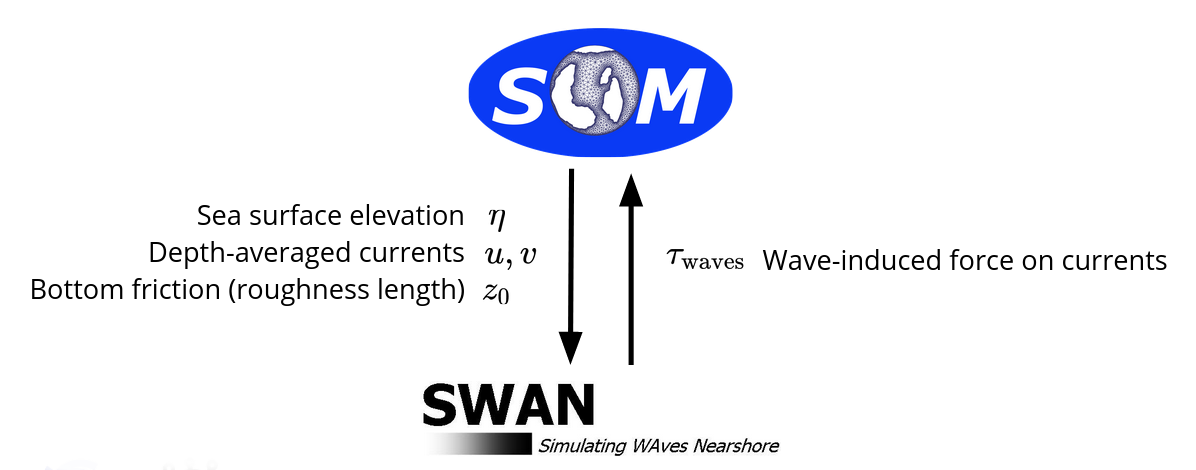
\includegraphics[width=.95\textwidth]{fig/coupling.png}
    \caption{Schematic illustration of the coupled SLIM+SWAN model.}
    \label{fig:coupling}
\end{figure}
 

%%%%%%%%%%%%%%%%%%%
% --- RESULTS --- %
%%%%%%%%%%%%%%%%%%%
\section{Results}

We first validated the reconstructed atmospheric fields of hurricane Irma as well the modelled currents and waves of our coupled model against fields measurements. We then use the validated model to simulate the transport of passive drifters in the Lower Keys during the passage of the hurricane. These drifters were advected by two sets of currents: (i) the currents from an uncoupled SLIM simulation of Irma (SLIM) and (ii) the currents modelled by the coupled SLIM+SWAN model (SLIM+SWAN). Furthermore, the depth-averaged Stokes drift was computed using our coupled model (Stokes\_C) and an uncoupled SWAN simulation of the hurricane (Stokes\_U). We then simulated the trajectories of passive drifters during the passage of the Irma in the Lower Keys using different combinations of these fields. These trajectories were finally compared to evaluate the impact of the wave-current interactions and the Stokes drift on the transport processes during a major hurricane.

\subsection{Model validation}

H*Wind winds and hybrid pressure field agree well with station measurements at Vaca Key station (Fig. \ref{fig:forcings}). The hybrid pressure field shows better agreement with observations than ERA-5 pressure as it successfully reproduces the storm depression. ERA-5 fields, on the other hand, fail to resolve the low pressure at the core of the hurricane due to their coarser grid, leading to an overestimation of 8 mbar of the storm depression. Both H*Wind and ERA-5 agree well with observed wind speeds although both data sets tend to slightly overestimate the width and intensity of the wind peak. However, H*wind profiles show a better match with the timing of the observed peak, as ERA-5 winds tend to anticipate it. H*wind also exhibits a slightly narrower peak in wind speed, which better agrees with observations.

\begin{figure}
    \centering
    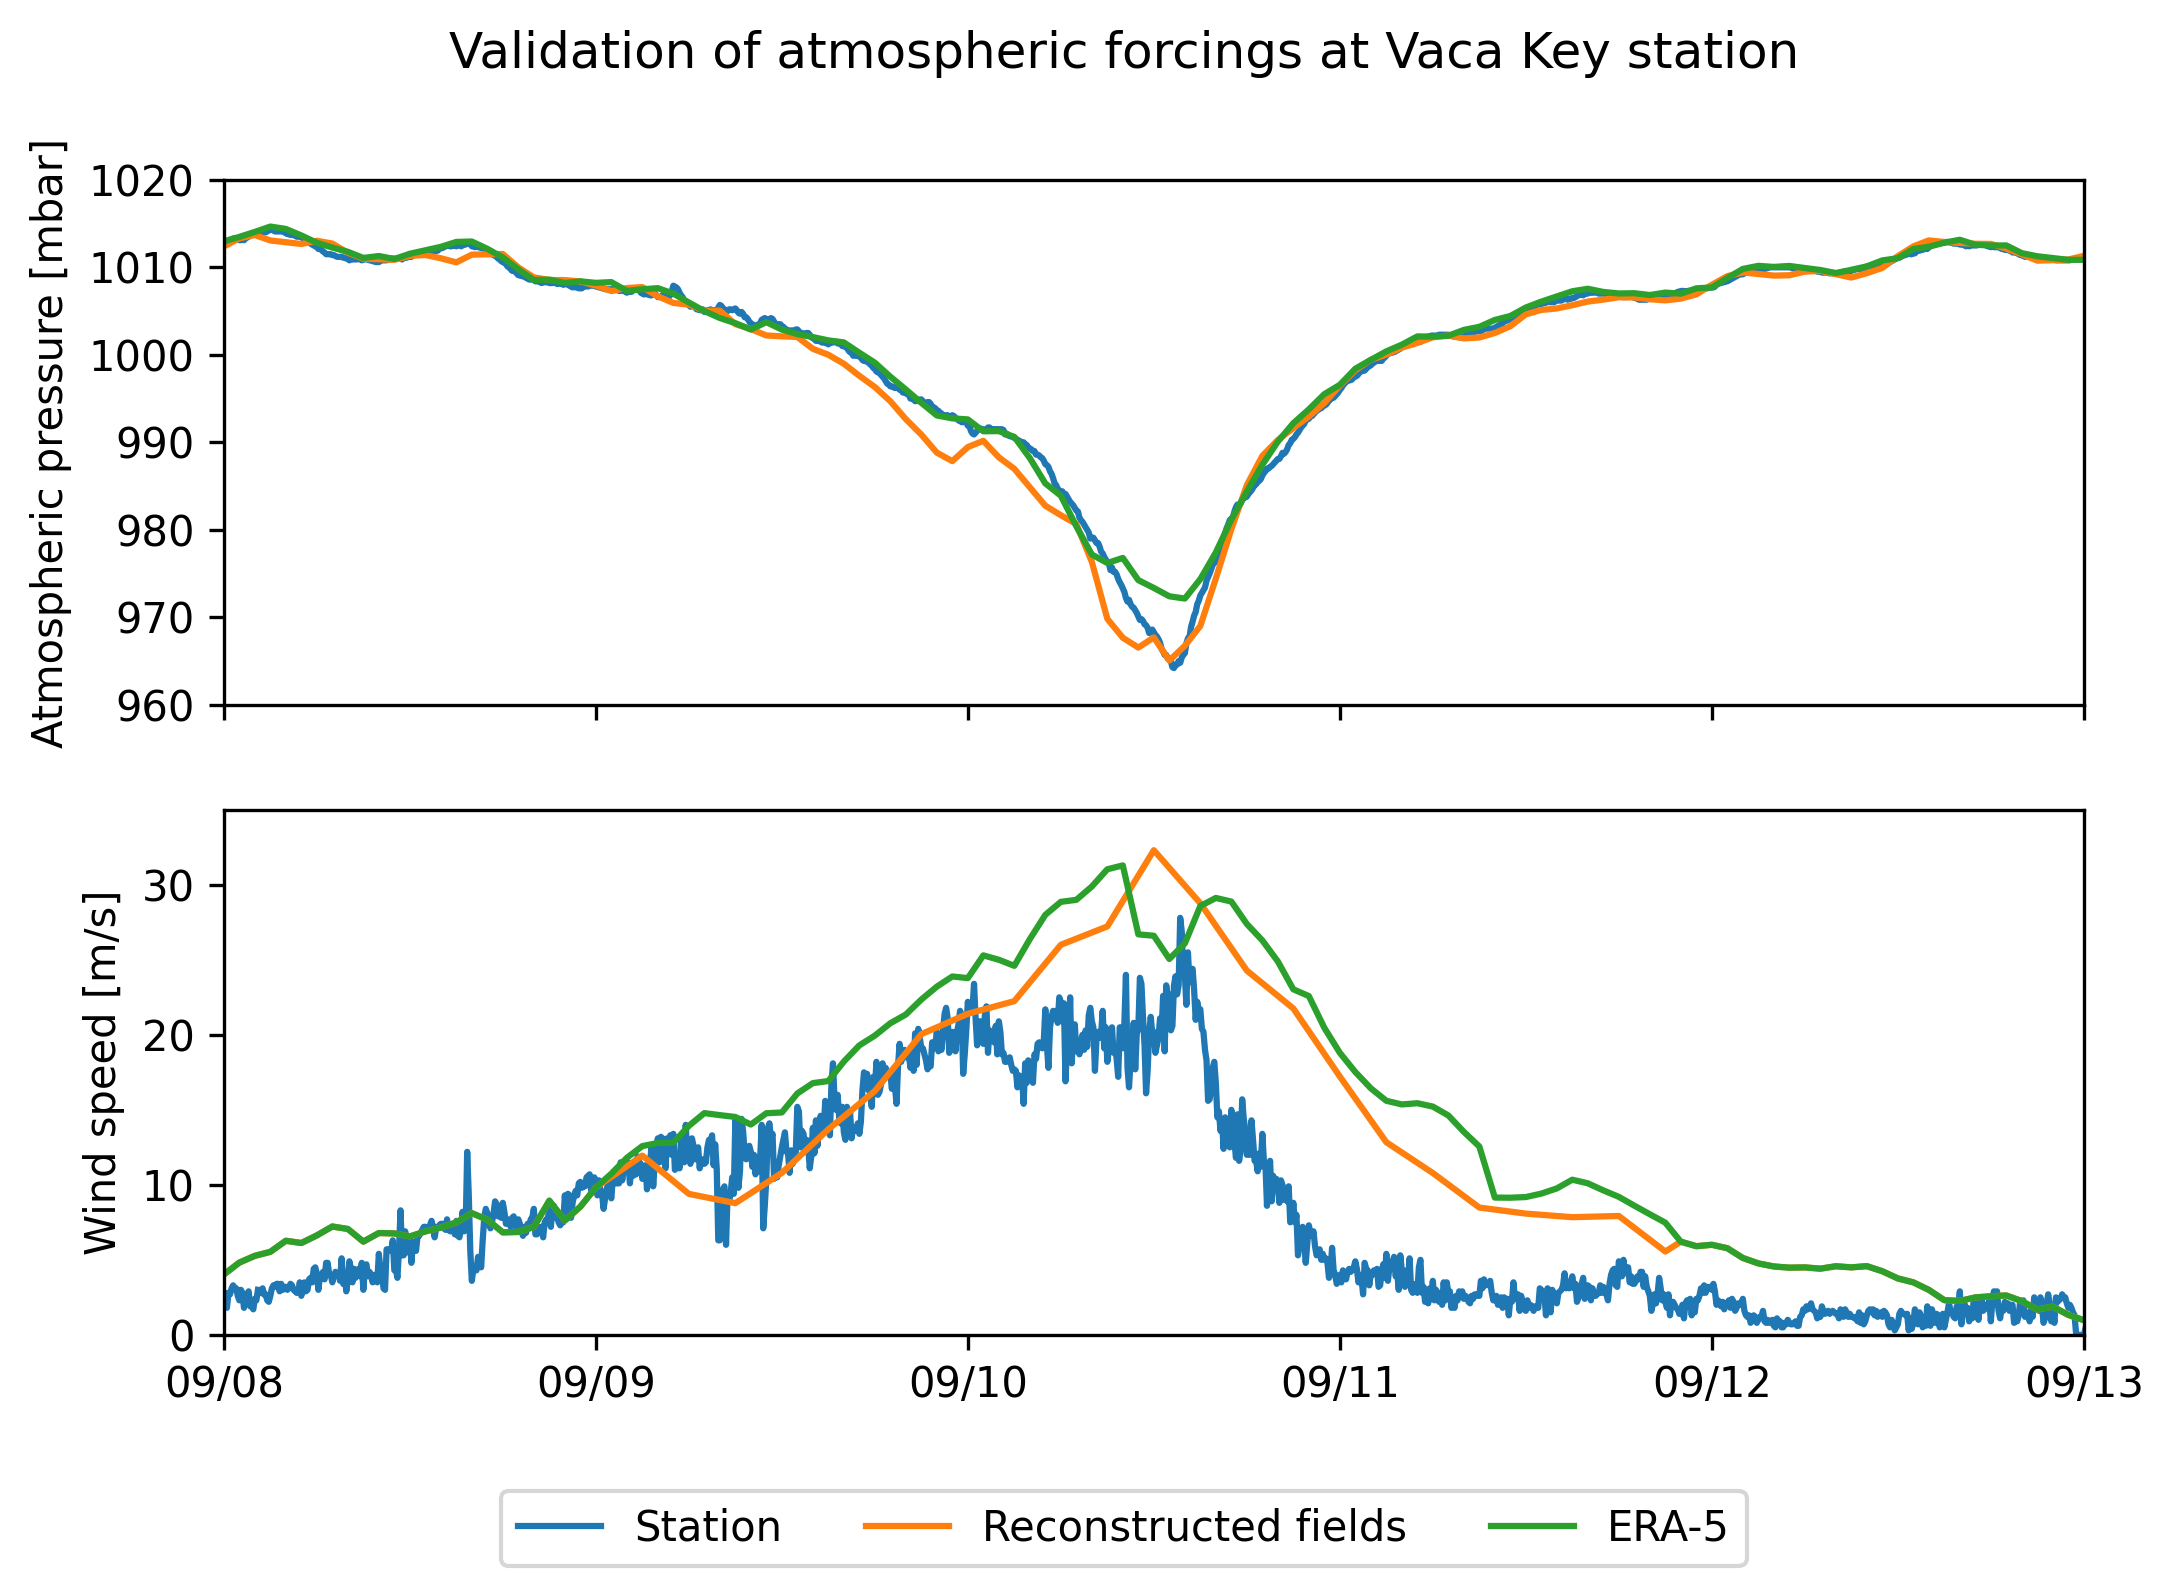
\includegraphics[width=.95\textwidth]{fig/validation_met_2.png}
    \caption{Comparison of reconstructed wind atmospheric pressure with field measurements and coarser ECMWF ERA-5 profiles at Vaca Key station. The generated hybrid atmospheric forcings better capture the observed storm depression while H*wind winds better match the measured peak in wind speed.}
    \label{fig:forcings}
\end{figure}

Hydrodynamic outputs of the coupled wave-current agree well with tide gauge (Fig. \ref{fig:sse}) and ADCP measurements (Fig. \ref{fig:uv}). The timing and amplitude of the storm surges are well reproduced by the coupled model, the largest model error being an overestimation of 18 cm of the elevation peak at Virginia Key. The fit is especially good at Naples, where both the positive and negative surges are captured by the coupled model with an error of less than 5 cm. This result is of interest as negative surges, although less studied, affect water exchanges between the estuaries and the coastal ocean and disturb the benthic ecosystems \citep{liu2020impacts}. Modelled 2D currents were validated against depth-averaged ADCP measurements at mooring station C10, C12 and C13 (Fig. \ref{fig:uv}). As in \cite{liu2020impacts}, we performed the vector correlation analysis of \cite{kundu1976ekman} to compare modelled and observed current velocity vectors. Correlation coefficients ($\rho$) between simulated and observed depth-averaged currents were 0.84, 0.74 and 0.73 at the C10, C12 and C13 locations, respectively. Average veering angles were computed as well and were below 12$^\circ$, as in \citep{liu2020impacts}. However, in our case, no clear tendency regarding modelled current behavior compared to observations was observed. As expected from a depth-averaged model, the best fit with observations is obtained at the shallowest mooring C10, located on the 25m isobath, with an average veering angle of 6$^\circ$. 

\begin{figure}
    \centering
    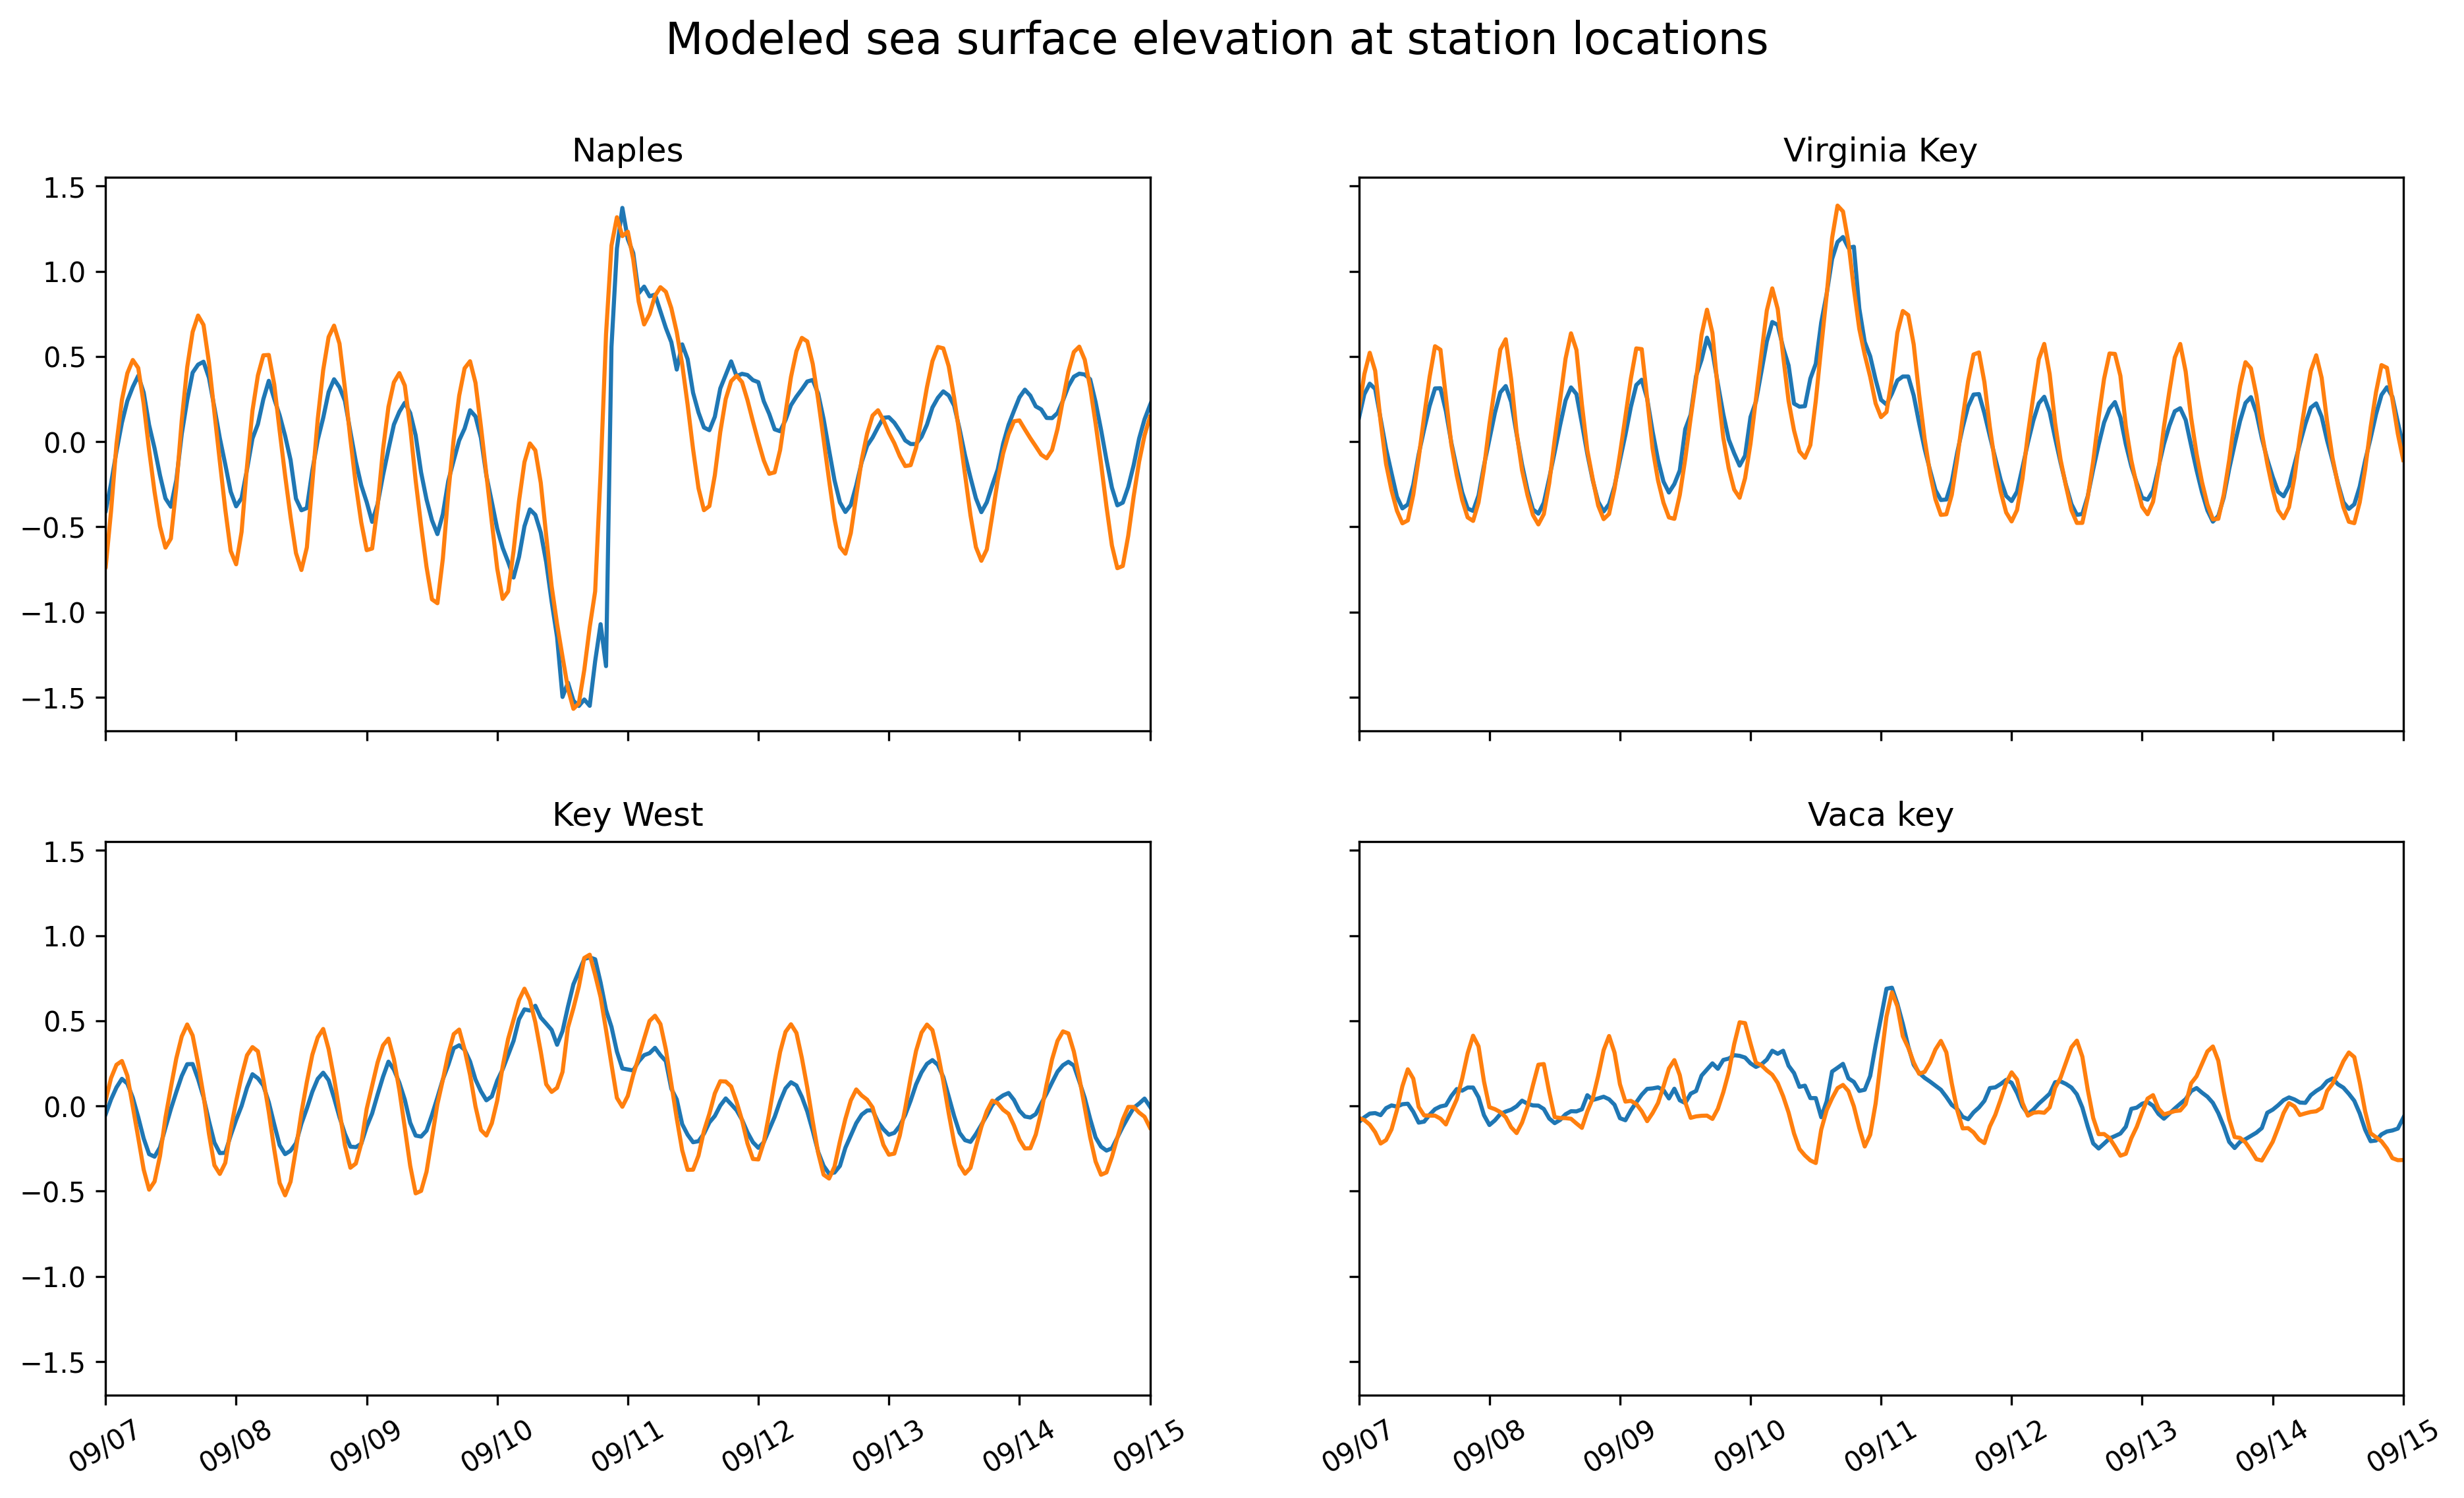
\includegraphics[width=\textwidth]{fig/elevation_with_map.png}
    \caption{Comparison of modelled sea surface elevation with all 4 tide gauge measurements (see Fig. \ref{fig:mesh}B for their location). Timing and amplitudes of the storm surges are well reproduced by the model}
    \label{fig:sse}
\end{figure}
\begin{figure}
    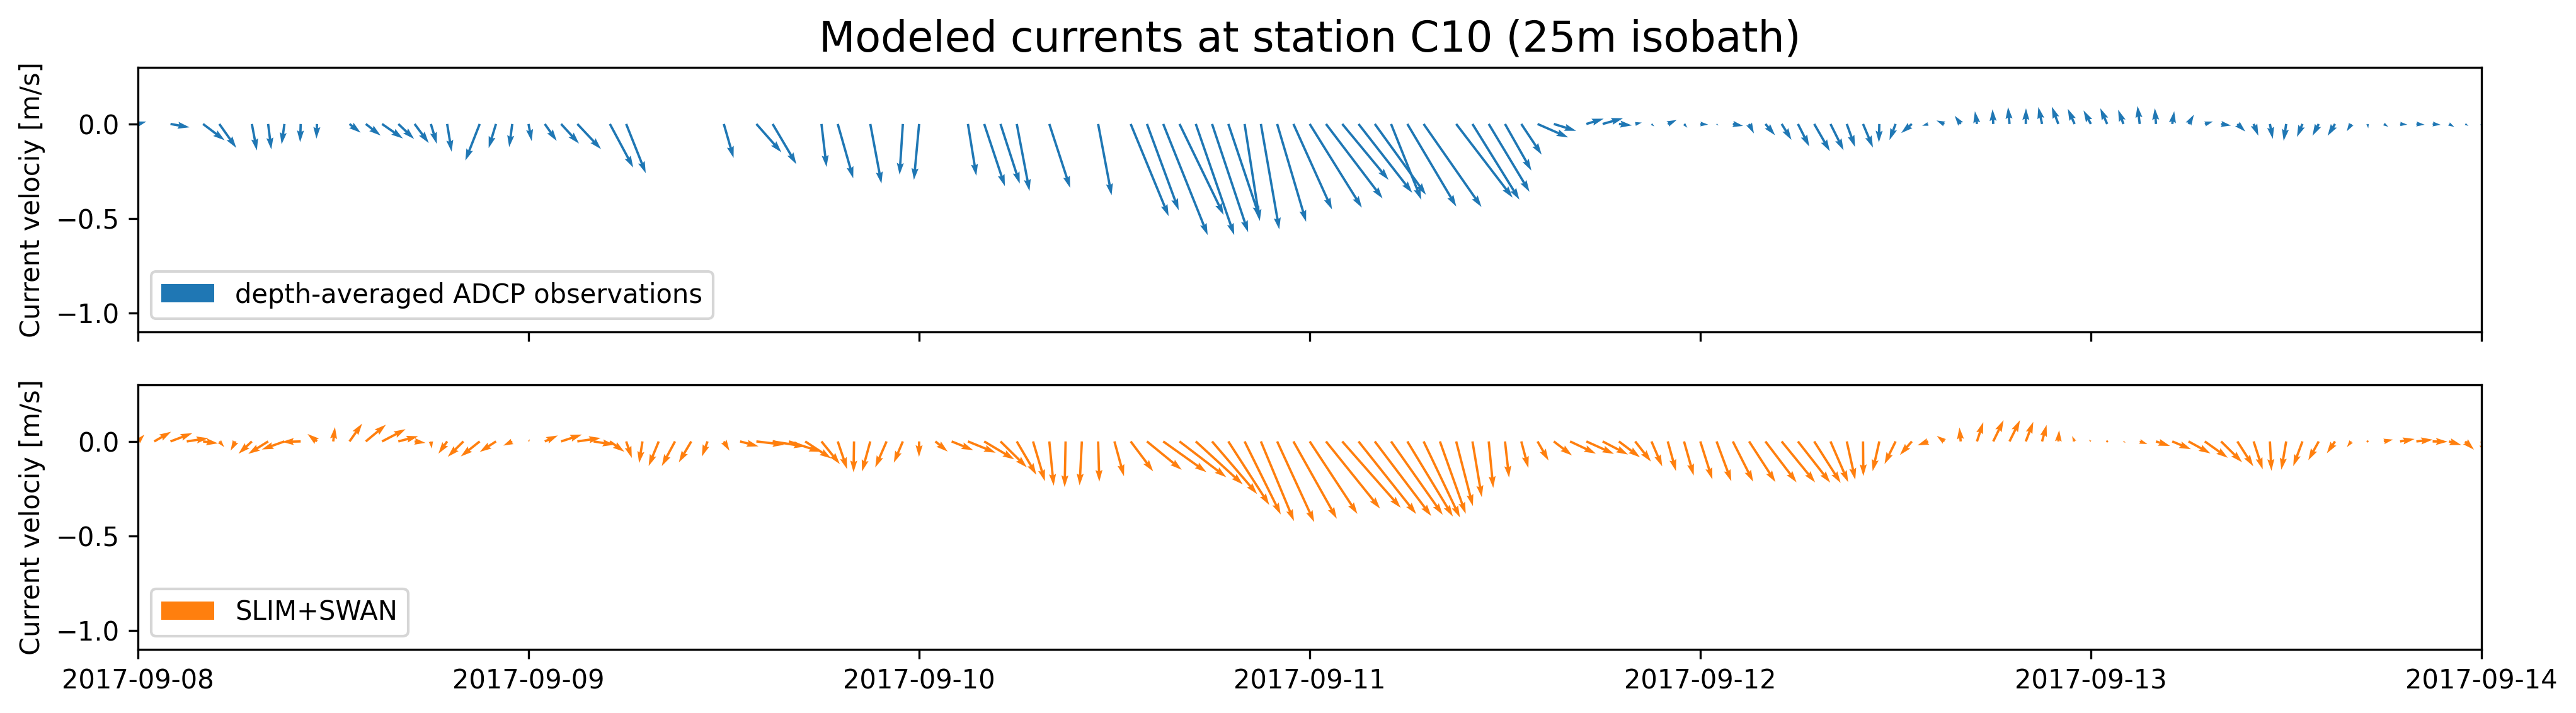
\includegraphics[width=\textwidth]{fig/validation_currents_C10_ww3.png}
    \caption{Comparison of modelled current velocity with observed velocity at mooring C10 (see Fig. \ref{fig:mesh}B for its location). Modelled current velocities agree well with observations, with a correlation coefficient of 0.83 and an average veering angle of $6^\circ$.}
    \label{fig:uv}
\end{figure}

The simulated significant wave height agrees well with observations on the WFS, where errors on the peak value do not exceed 5\% (Fig. {fig:waves}). On the East Florida Shelf, errors are slightly larger and reach 20\%. Although the model outputs agree well with observations, a lag in significant wave height is observed for all 4 buoys. Moreover, the peak in significant wave height tends to be underestimated at buoys 41113 and 41114, located on the East Florida Shelf. Other wave parameters were better reproduced by the model on the WFS as well (see buoy 42036 in Fig. \ref{fig:waves}). This good fit on the WFS is not surprising as the parameters used for wind energy input and whitecapping dissipation were based on the calibration performed by \cite{siadatmousavi2011evaluation} on the Northern Gulf of Mexico. Wind-induced wave growth might therefore be underestimated on the eastern shelf. Consequently, incident wave do not receive enough energy to grow after breaking on the bank boundary, leading to an underestimation of the significant wave height at the location of the buoys. Nonetheless, as this study focused on the wave produced by Irma, that made landfall on the western coasts of Florida, the use of parameterizations calibrated for the Gulf of Mexico seems reasonable.

\begin{figure}
    \centering
    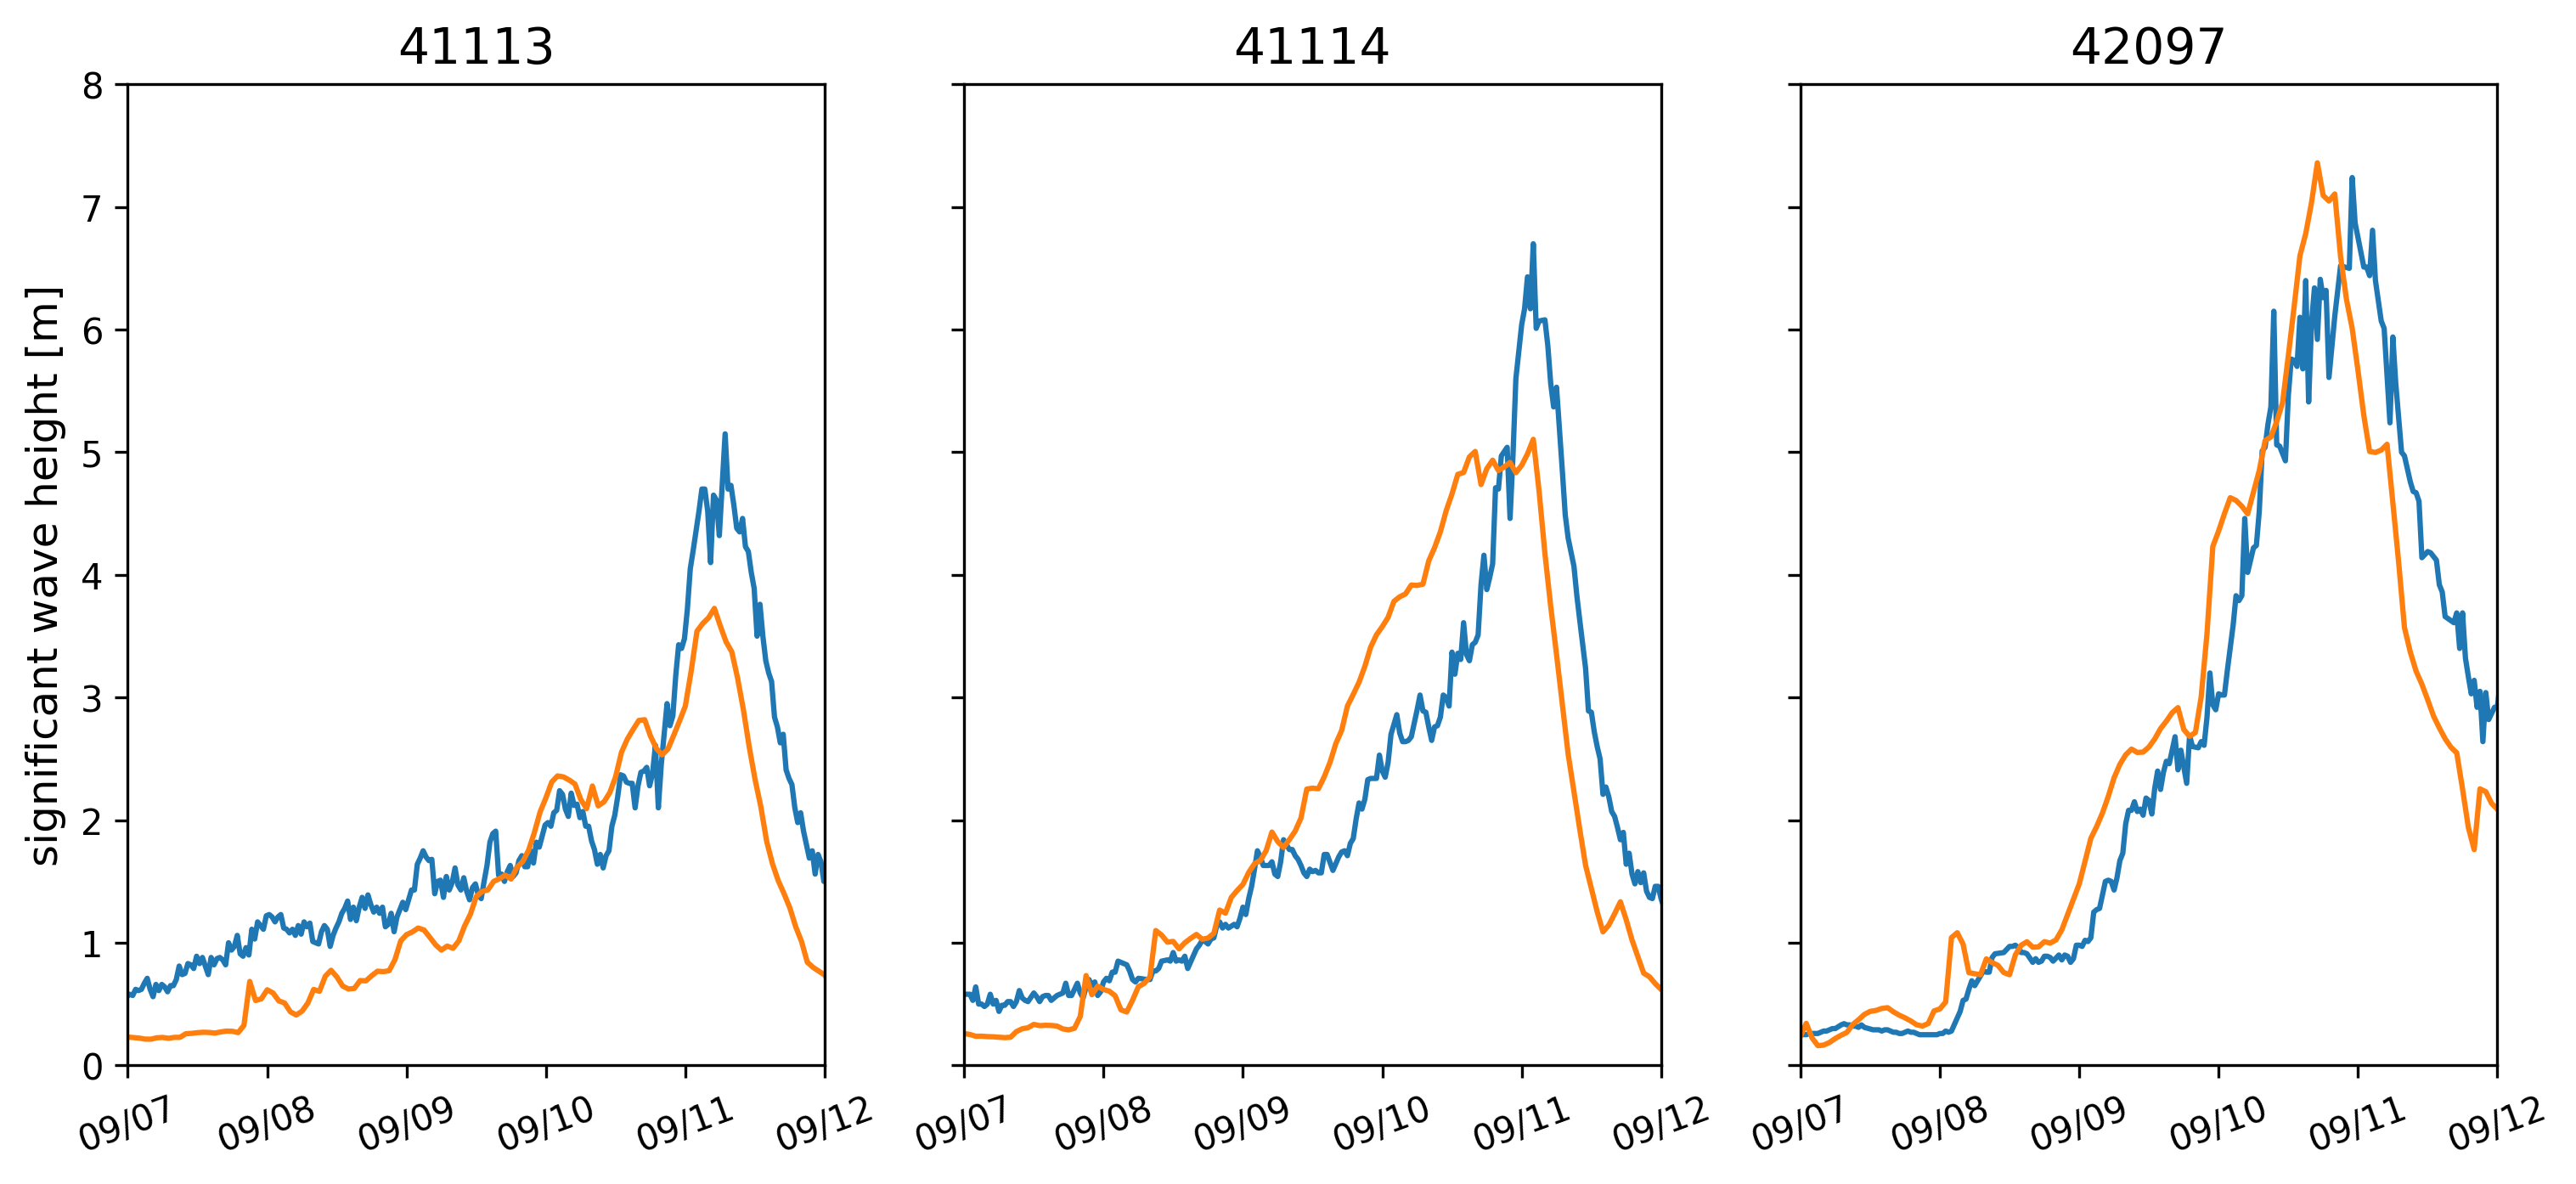
\includegraphics[width=\textwidth]{fig/hsig_with_map_ww3.png}
    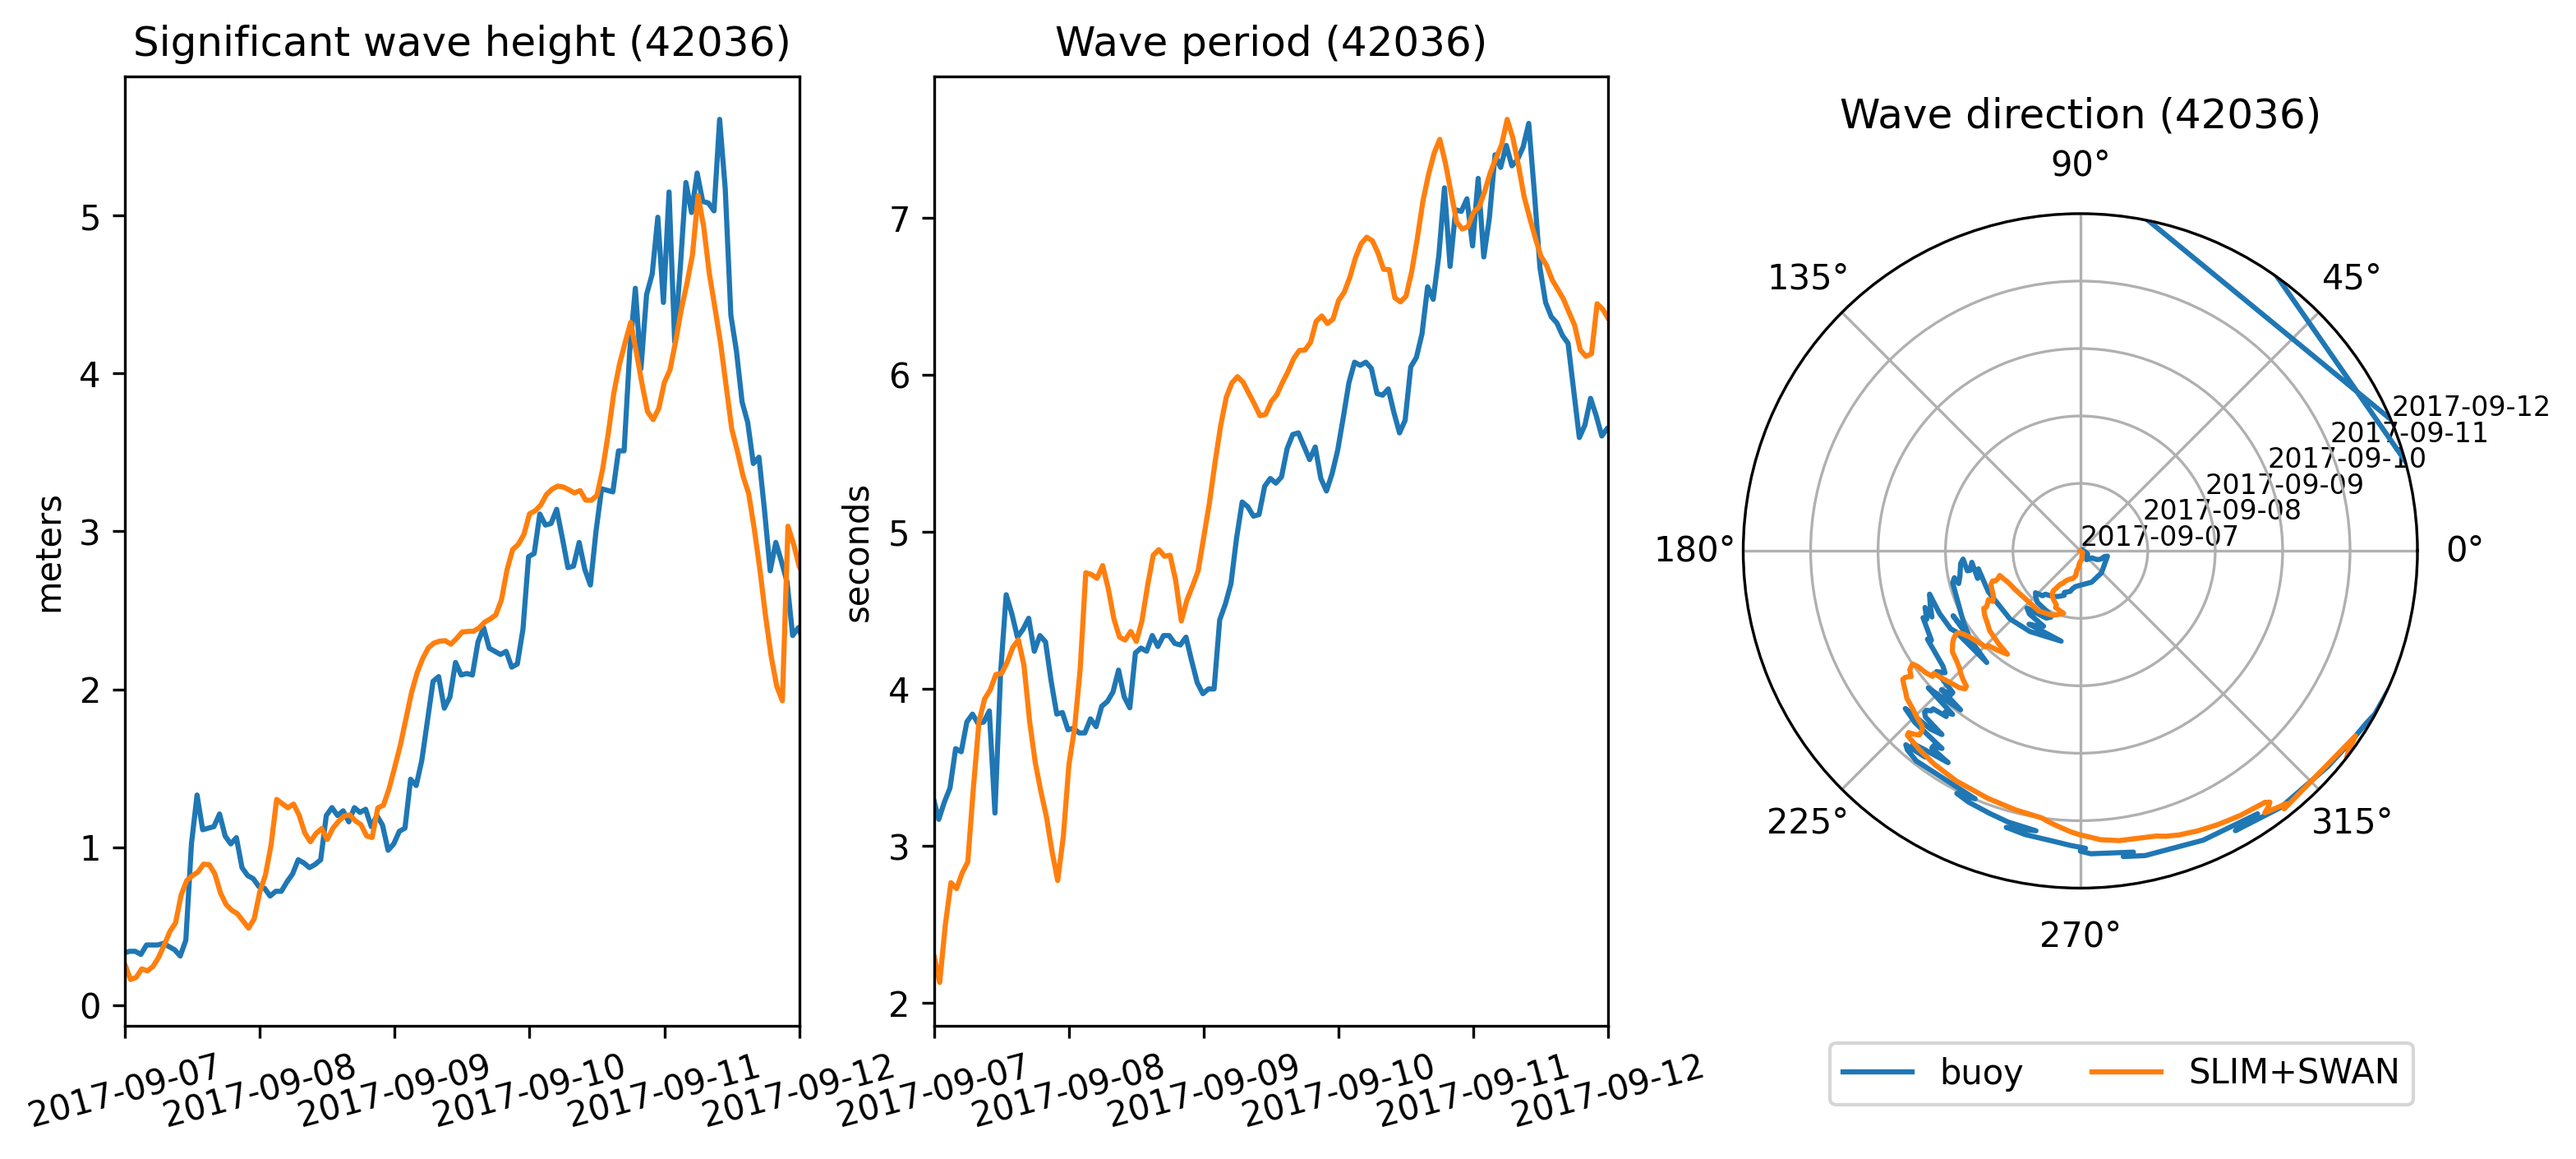
\includegraphics[width=\textwidth]{fig/waves_ww3_5km-00002.png}
    \caption{Comparison of modelled wave parameters with observation at the 4 buoys location (locations shown in Fig. \ref{fig:mesh}B). Modelled significant wave height agrees well with field measurement. As model parameters were calibrated for the Northern Gulf of Mexico, observations are better reproduced at buoys located on the WFS, as illustrated for buoy 42036}
    \label{fig:waves}
\end{figure}

\subsection{Impact of waves on currents and transport}

We evaluated the impact of wave-current interactions on modelled currents during the passage of Irma in the Lower Keys, between Sept. 7 and 13, 2017. First, we computed the maximum difference between currents modelled by SLIM and SLIM+SWAN during this period (Fig. \ref{fig:diff}A). The largest differences in current speed were observed over the reefs, on the shelf break and around islands. They can locally reach 1 m/s, with the coupled model SLIM+SWAN yielding the largest amplitudes. The regions where the differences are the largest experience the largest wave-induced stress {\boldmath$\tau$}$_\text{wave}$ (\ref{fig:diff}B), as wave breaking and wave slowing down over rough seabed induce variations of the wave radiation stress \citep{longuet1964radiation}. Wave-induced differences in current speed were amplified by the action of the wind stress {\boldmath$\tau$}$_\text{wind}$ (Fig. \ref{fig:diff}C). Wind speeds were larger in the front right quadrant of the hurricane \citep{zedler2009ocean}, yielding larger differences on the right-hand side of the storm trajectory. This is especially clear in the area between the Florida Keys and the Everglades, where relatively small values of {\boldmath$\tau$}$_\text{wave}$ nonetheless produce current speed differences of up to 0.5 m/s because of the wind stress.

\begin{figure}
    \centering
    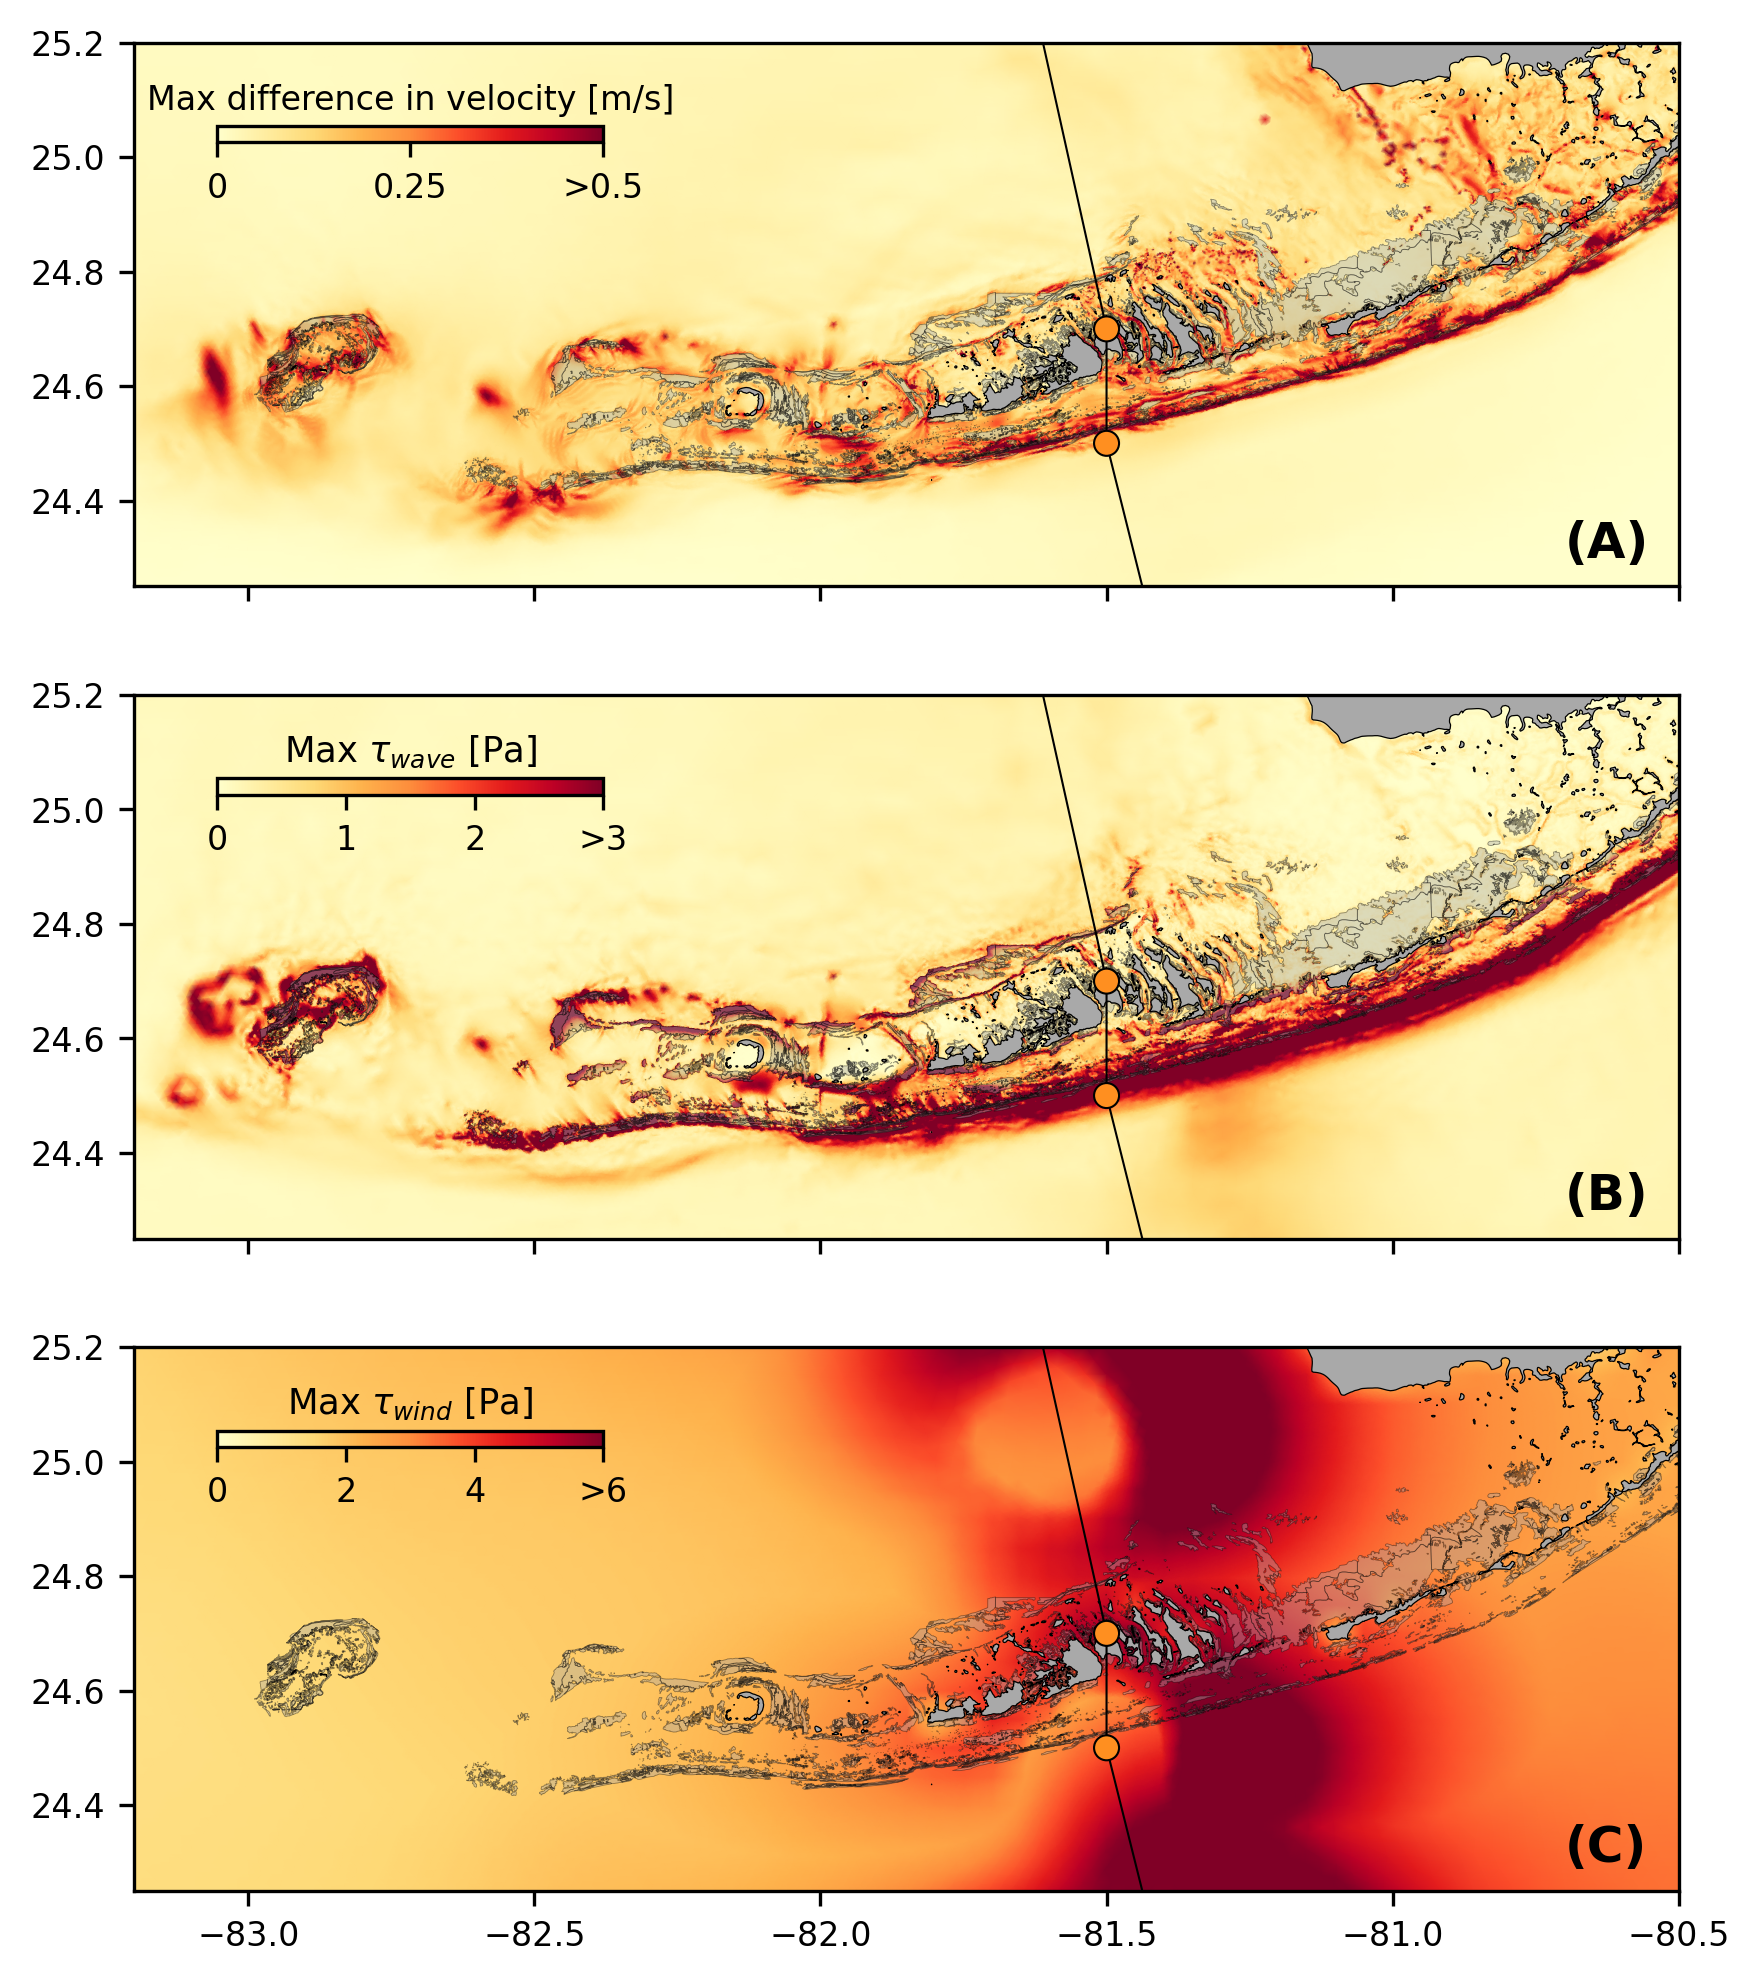
\includegraphics[width=\textwidth]{fig/max_diff_reefs.png}
    \caption{Maximum difference between SLIM and SLIM+SWAN currents (\textbf{A}) during the passage of Irma in the Lower Florida Keys, along with the maximum wave radiation stress gradient {\boldmath$\tau$}$_\text{wave}$ (\textbf{B}) and wind stress {\boldmath$\tau$}$_\text{wind}$ (\textbf{C}) generated by the hurricane. Wave-induced stress yields difference larger than 0.5 m/s in current velocities. These wave-induced differences in currents were amplified by the action of the asymetric wind profile of Irma, with larger differences occurring on the right of the storm trajectory}
    \label{fig:diff}
\end{figure}

To quantify the impact of these differences in the velocity fields, we compared the trajectories of passive particles advected by the uncoupled SLIM and coupled SLIM+SWAN currents during the passage of Irma in the Lower Keys (Fig. \ref{fig:traj}). Particles were released on the inner and outer shelves in the areas highlighted by red and blue circles in Fig. \ref{fig:traj}A on 7 September and then tracked until 15 September. These areas were constructed using backtracking methods \citep{dobbelaerereport} to ensure that the release particles would intersect the path of Irma during its passage in the Florida Keys. We first defined two 25km$^\text{2}$ circular regions on the trajectory of the hurricane (see red and blue circles in Fig. \ref{fig:traj}A). Particles within these two regions were then tracked backward in time using uncoupled SLIM currents from the exact time of the passage of the hurricane until the 7th of September. Their positions at the end of the backward simulation (see red and blue particle clouds in Fig. \ref{fig:traj}) corresponds to the initial condition of the forward transport simulations described below. 

We compared the trajectories of particles originating from these regions and advected forward in time by different sets of currents: (i) uncoupled SLIM currents alone; (ii) coupled SLIM+SWAN currents; (iii) SLIM currents with the addition of the depth-averaged Stokes drift computed by the coupled wave model (Stokes\_C); (iv) SLIM+SWAN currents with Stokes\_C; and (v) SLIM currents with the depth-averaged Stokes drift computed by the uncoupled wave model (Stokes\_U). Particles trajectories are compared by computing the distances between the centers of mass of the particle clouds through time. Here are our main observations \emphc{(this needs to be improved, feedback is welcome!)} : 
\begin{itemize}
    \item The impact of wave-current interactions is most important during the passage of the hurricane but negligible during the rest of the simulated period. This is clear when comparing the clouds of particles advected by SLIM and SLIM+SWAN on the outer shelf. The distance between the centers of mass reaches 5 km during the passage of Irma but tends to zero during the rest of the simulated period.
    \item The impact of the Stokes drift is larger than the impact of the wave-current interactions on the inner shelf. The difference between the centers of mass does not exceed about 1 km for SLIM vs SLIM+SWAN but reaches about 5 km for SLIM vs SLIM+Stokes\textunderscore C and SLIM+SWAN+Stokes\textunderscore C. On the outer shelf, the currents are more intense and the impact the wave-current coupling during the passage of the hurricane is sufficient to generate a difference between the two clouds of particles that keeps on increasing after the passage of the hurricane. The impact of the Stokes drift remains however larger than the impact of the wave-current coupling. This difference between the inner and outer shelf can be explained by the sheltering of the inner shelf due to reefs and islands as well as wave breaking on the shelf break. The inner shelf hence experiences weaker waves and weaker currents, and hence also weaker and more localised transport. 
    \item On the inner shelf, the distance between the centers of mass of the particle clouds stabilizes after the passage of the hurricane while this distance keeps increasing during a couple of days after the passage of the hurricane on the outer shelf under the action of the Stokes drift. This shows the strong impact of wave-induced transport in the open ocean. 
    \item Impact of Stokes drift and wave-current interactions weaker on the inner shelf. Max. distance of about 5 km between the centers of mass of the clouds of particles compared to 30km on the outer shelves
    \item The fact that SLIM+Stokes\_C vs. SLIM+Stokes\_U keeps increasing on the outer shelf after the passage of the hurricane shows the impact of the strong current velocities of the FC on the modelled Stokes drift
    \item Nonetheless, the differences between the coupled and uncoupled Stokes drifts remains relatively small with a maximum value of 2 km between the centers of mass of the simulated particle clouds. Furthermore, as SLIM vs SLIM+SWAN+Stokes and SLIM vs. SLIM+Stokes\_C show similar values on the inner shelf, this suggests that the combination of currents and Stokes drifts produces sufficiently accurate results on sheltered shallow areas such as the WFS. However, neglecting the wave-current interactions leads to differences of up to 5 km in modelled particle trajectories on the outer shelf. 
\end{itemize}

\begin{figure}
    \centering
    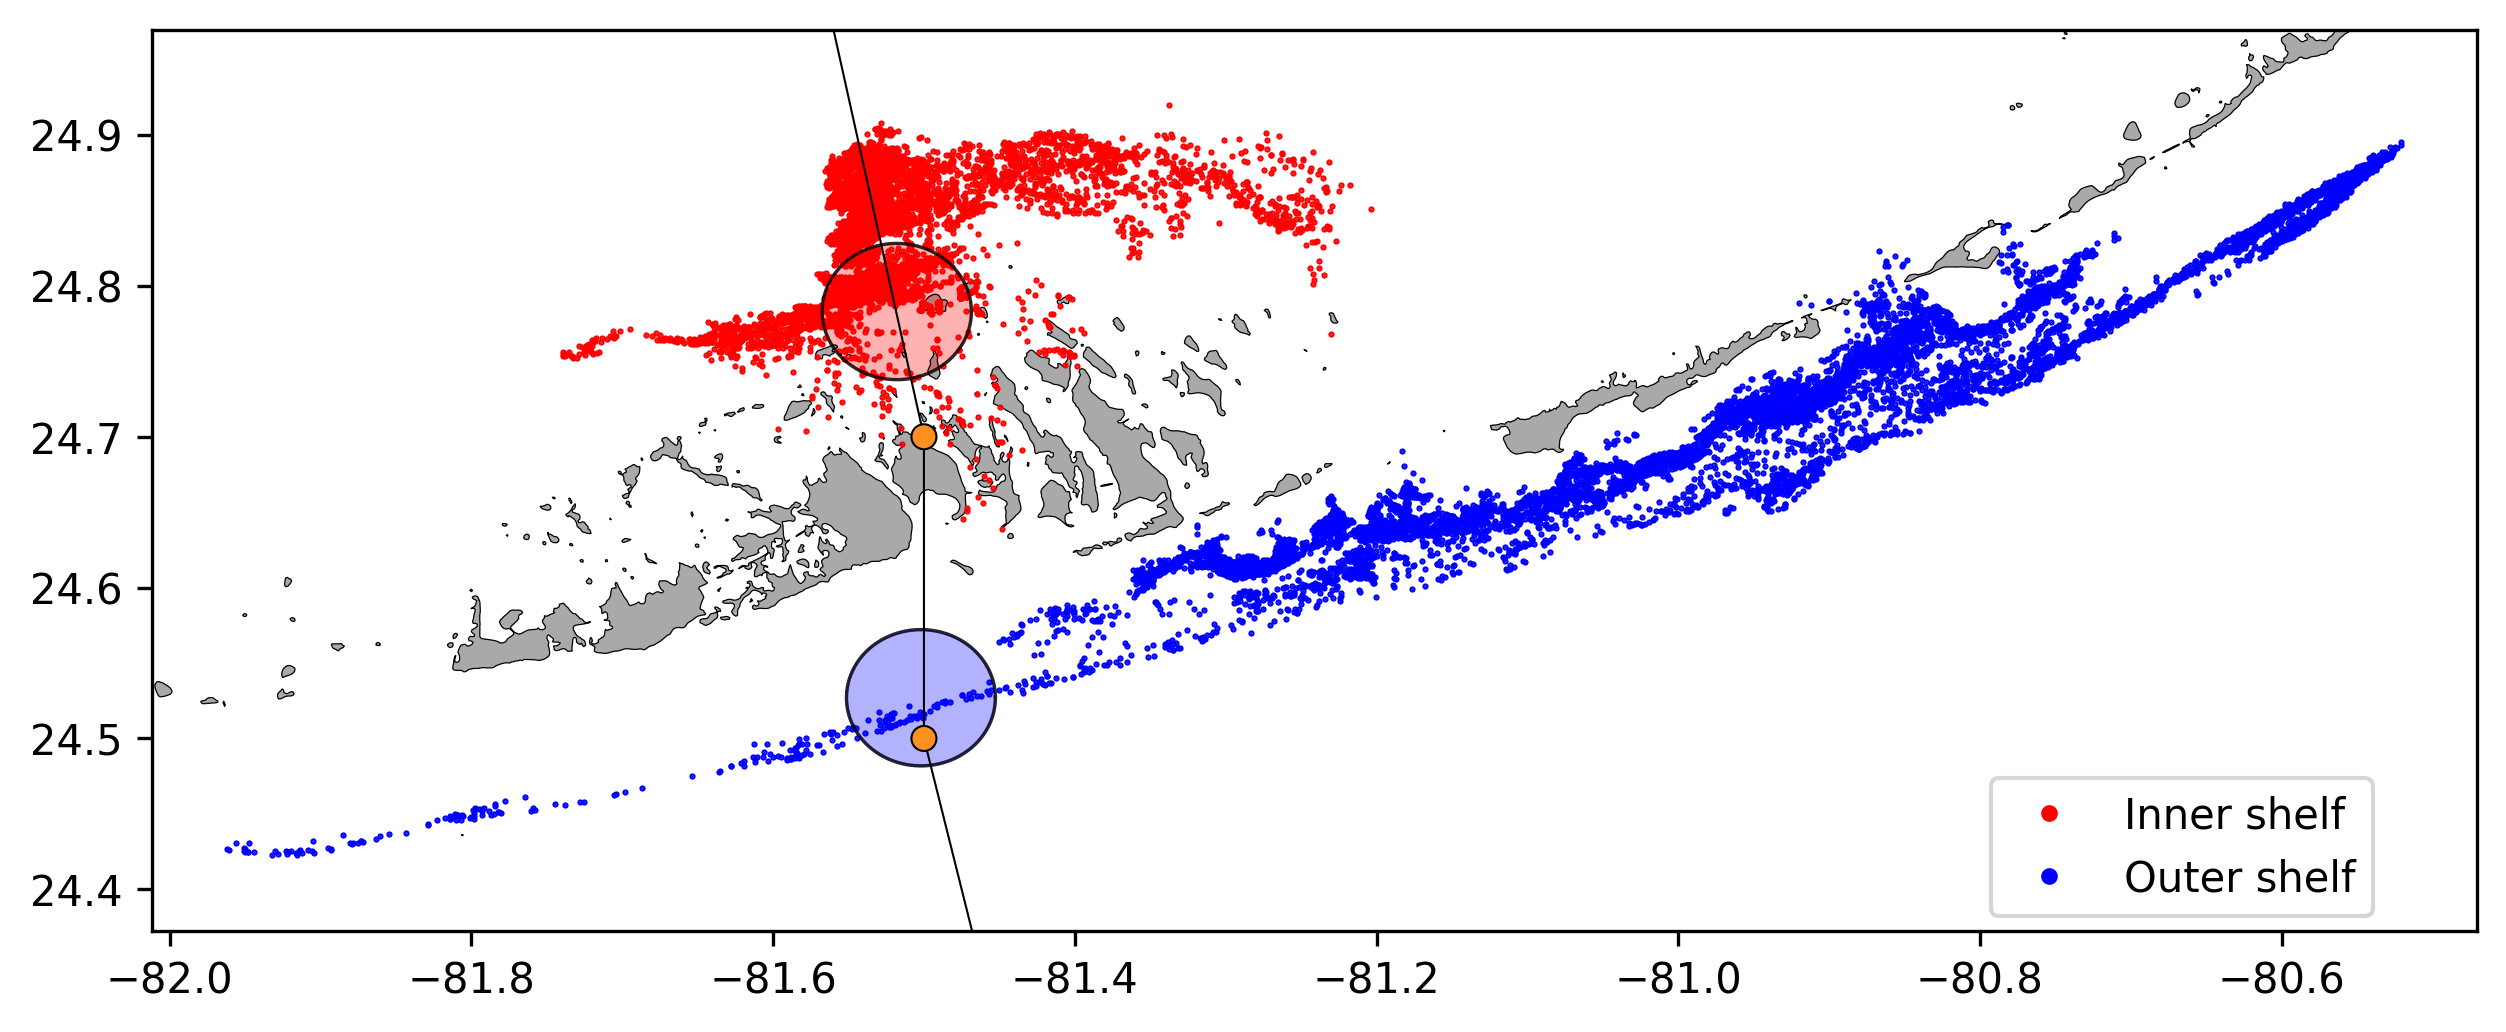
\includegraphics[width=.85\textwidth]{fig/inner_outer_regions.png}
    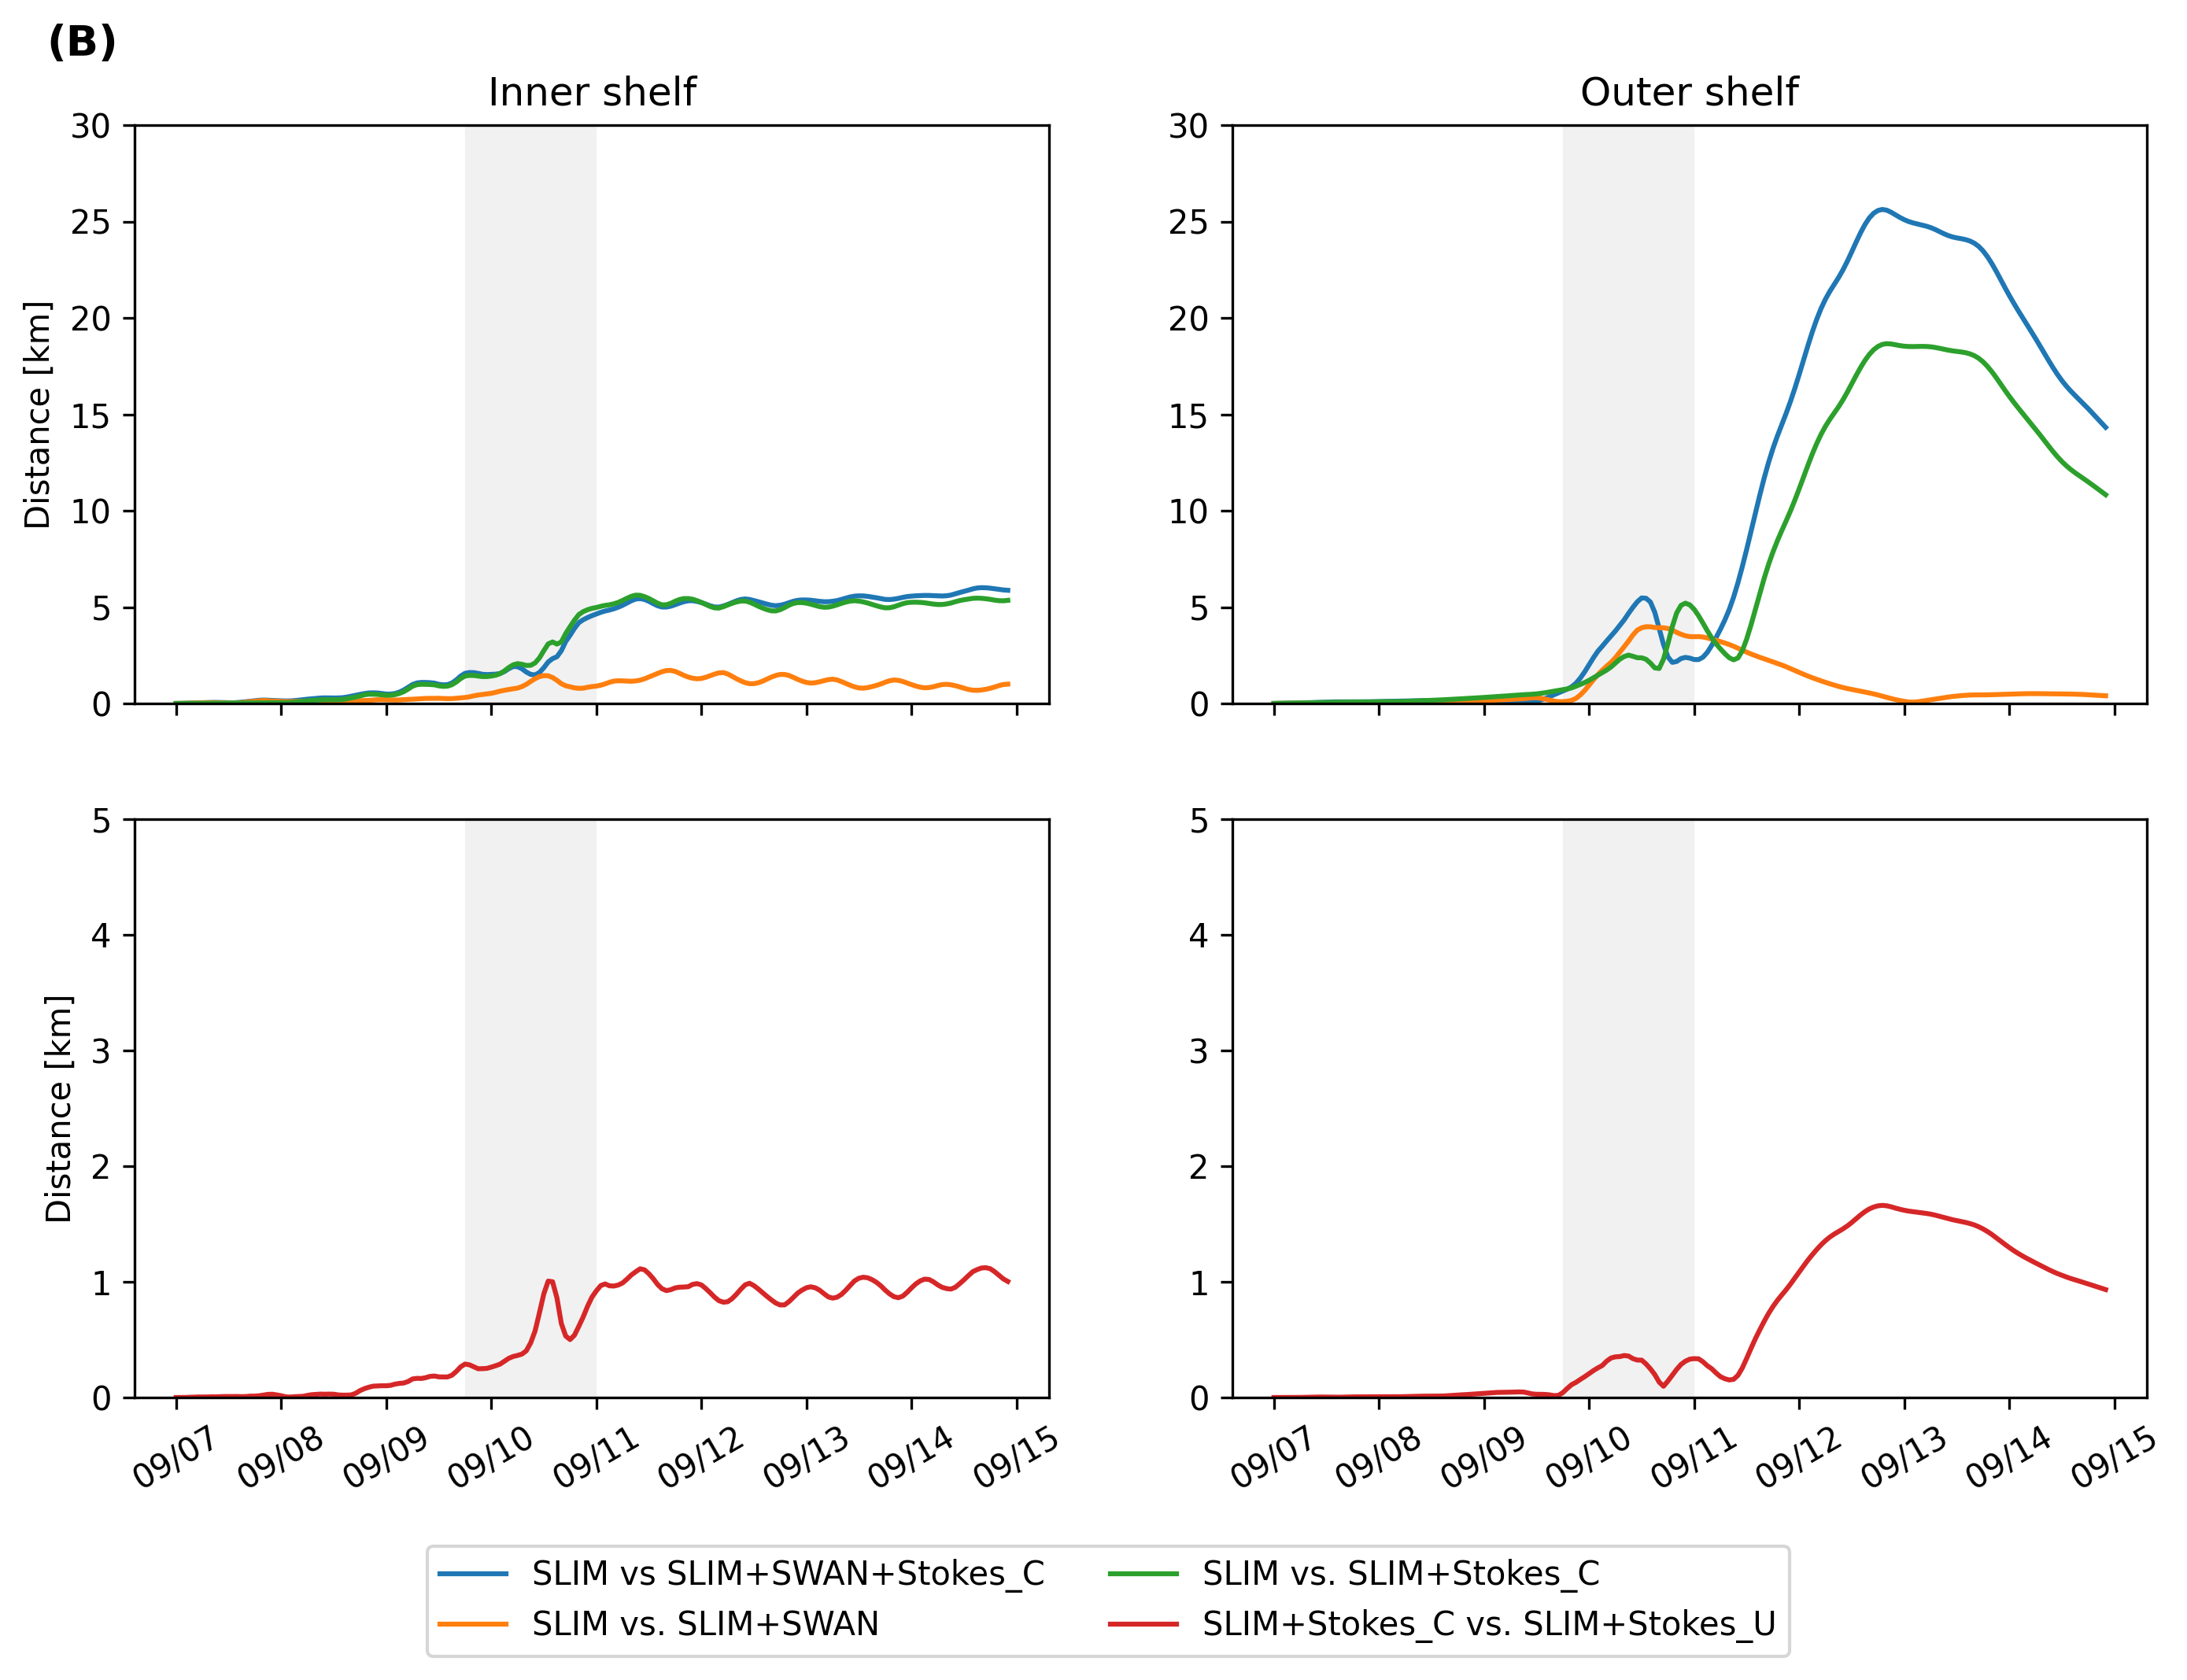
\includegraphics[width=.99\textwidth]{fig/inner_outer.png}
    \caption{\textbf{A}: Release regions of the passive particles on the inner and outer shelves (red and blue clouds) obtained by backtracking particles released in the red and blue circular areas during the passage of Irma \emphc{(add a black border to the circles to better see them)}. \textbf{B}: Difference between the centers of mass of the particle clouds released from the regions highlighted in \textbf{A} and advected by different combinations of coupled and uncoupled velocity fields.}
    \label{fig:traj}
\end{figure}

% === DISCUSSION === %
\section{Discussion and conclusions}

Impact of waves on coral connectivity

Ability of wave model to correctly capture gradient in significant wave height due to current-waves interactions under tropical cyclones depends on:
\begin{itemize}
    \item Broad perspective $\Rightarrow$ not limited to FL
    \item Mention search and rescue
    \item However, ignoring waves in storm conditions could result in significant inaccuracies in modelled trajectories, as illustrated in the case of release region 2 in Fig. \ref{fig:traj}
    \item Spatial (10km $\to$ 5km) and spectral (36 dir. $\to$ 48 dir.) resolution \citep{hegermiller2019wave}
    \item Directional spreading of incident waves \citep{villas2020wave}
\end{itemize}

\section*{Conflict of Interest Statement}
The authors declare that the research was conducted in the absence of any commercial or financial relationships that could be construed as a potential conflict of interest.

\section*{Author Contributions}
  
\section*{Funding}

\section*{Acknowledgments}
Computational resources were provided by the Consortium des \'Equipements de Calcul Intensif (\textsc{c\'eci}), funded by the \textsc{f.r.s.-fnrs} under Grant No. 2.5020.11. Thomas Dobbelaere is a PhD student supported by the Fund for Research training in Industry and Agriculture (\textsc{FRIA}/\textsc{FNRS}).

\section*{Supplementary Material}
The Supplementary Material for this article is attached to the submitted document.

% === BIBLIOGRAPHY === %
% \bibliographystyle{frontiersinSCNS_ENG_HUMS} 
\bibliographystyle{apalike}
\bibliography{./biblio.bib}

%%% Make sure to upload the bib file along with the tex file and PDF
%%% Please see the test.bib file for some examples of references

% \appendix
% \section*{Appendix}
% \renewcommand{\thesection}{A}
% \setcounter{figure}{0}
% \renewcommand{\thefigure}{\thesection\arabic{figure}}

\end{document}
